\chapter{High Multiplicity Jets at \texttt{ATLAS}}
\label{chap:ATLAS}

	Show the ATLAS pure jets analysis and talk a bit about the issues with running the damn thing.  Talk about the conclusions about BFKL-like dynamics

	\begin{figure}[H]
		\centering
		\begin{subfigure}[b]{0.48\textwidth}
			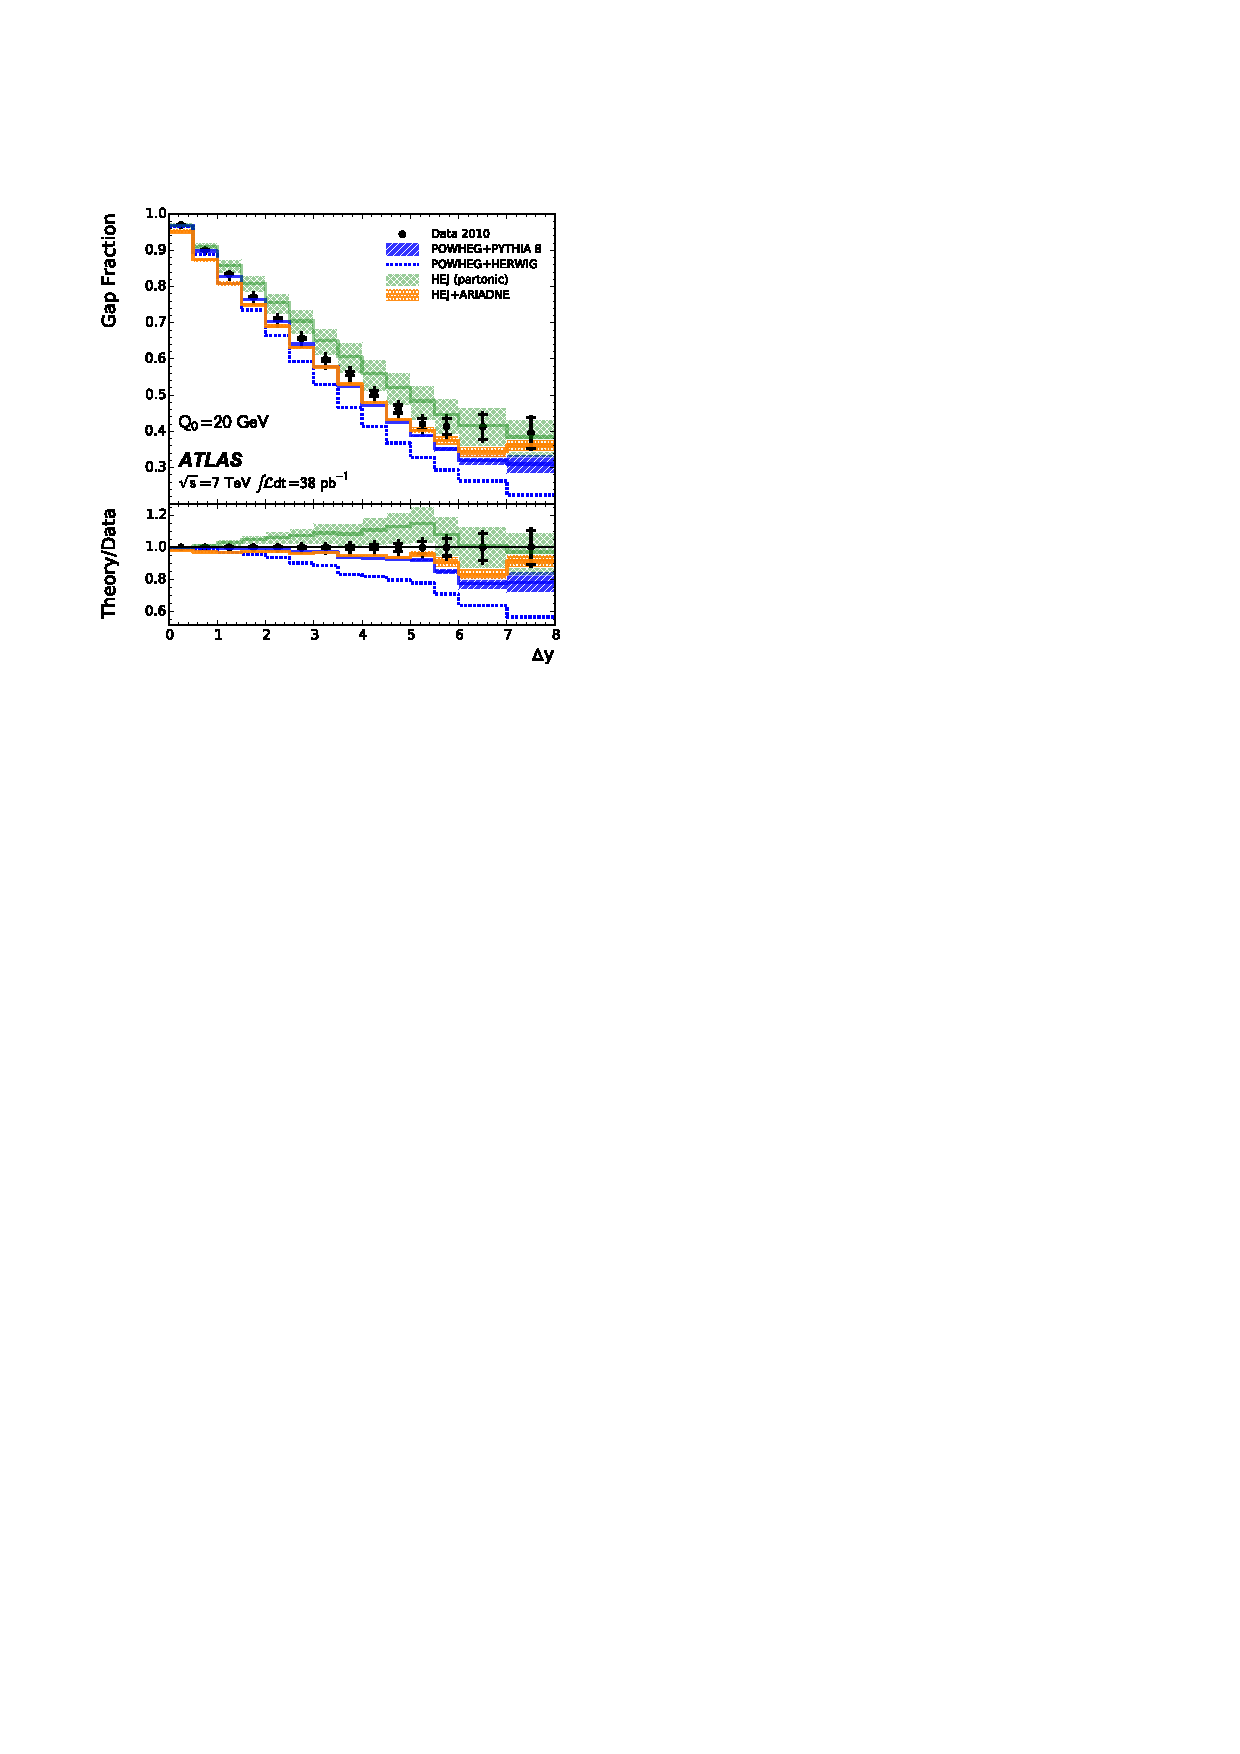
\includegraphics[width=\textwidth, height=1.0\textwidth]{pureJets3a}
			\caption{}
			\label{fig:}
		\end{subfigure}
		~
		\begin{subfigure}[b]{0.48\textwidth}
			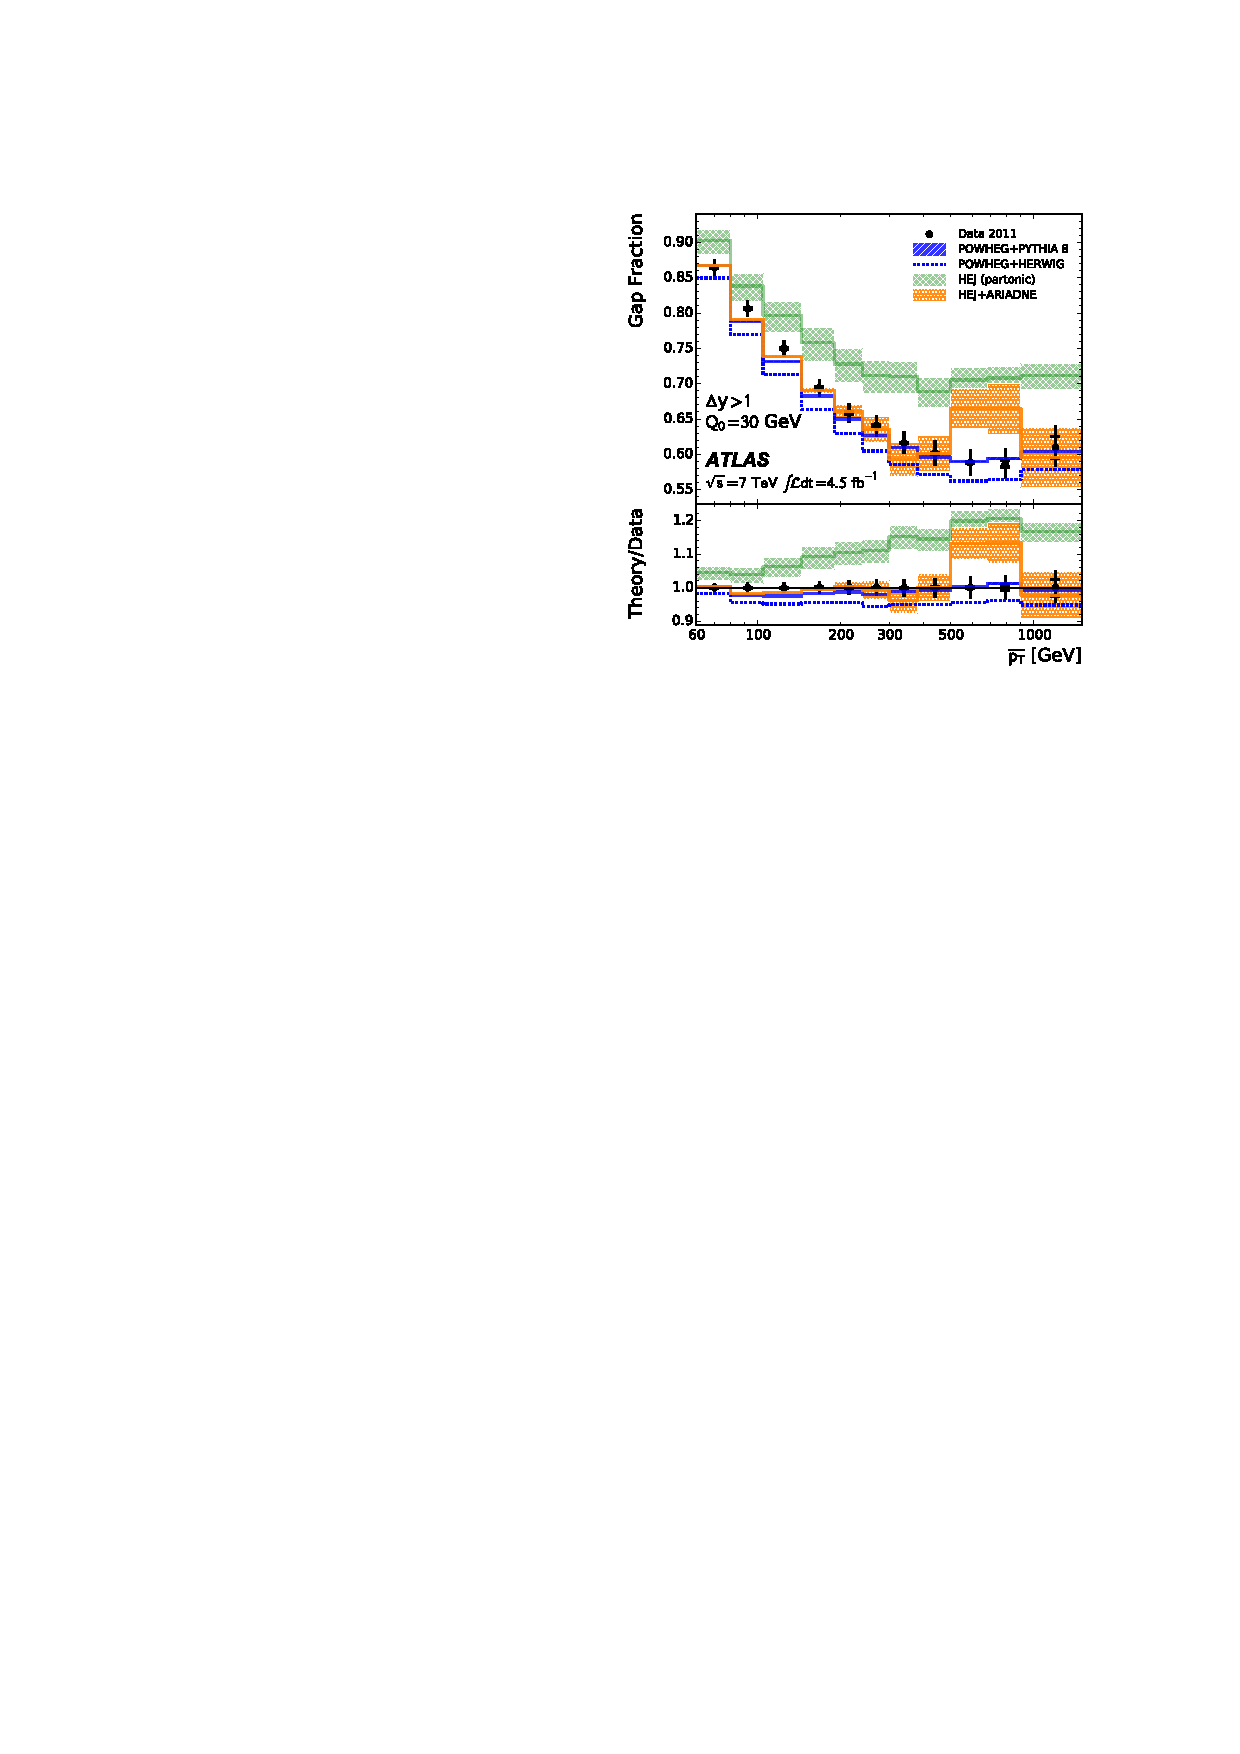
\includegraphics[width=\textwidth, height=1.0\textwidth]{pureJets3b}
			\caption{}
			\label{fig:}
		\end{subfigure}
		\caption{}
		\label{fig:}

		\begin{subfigure}[b]{0.48\textwidth}
			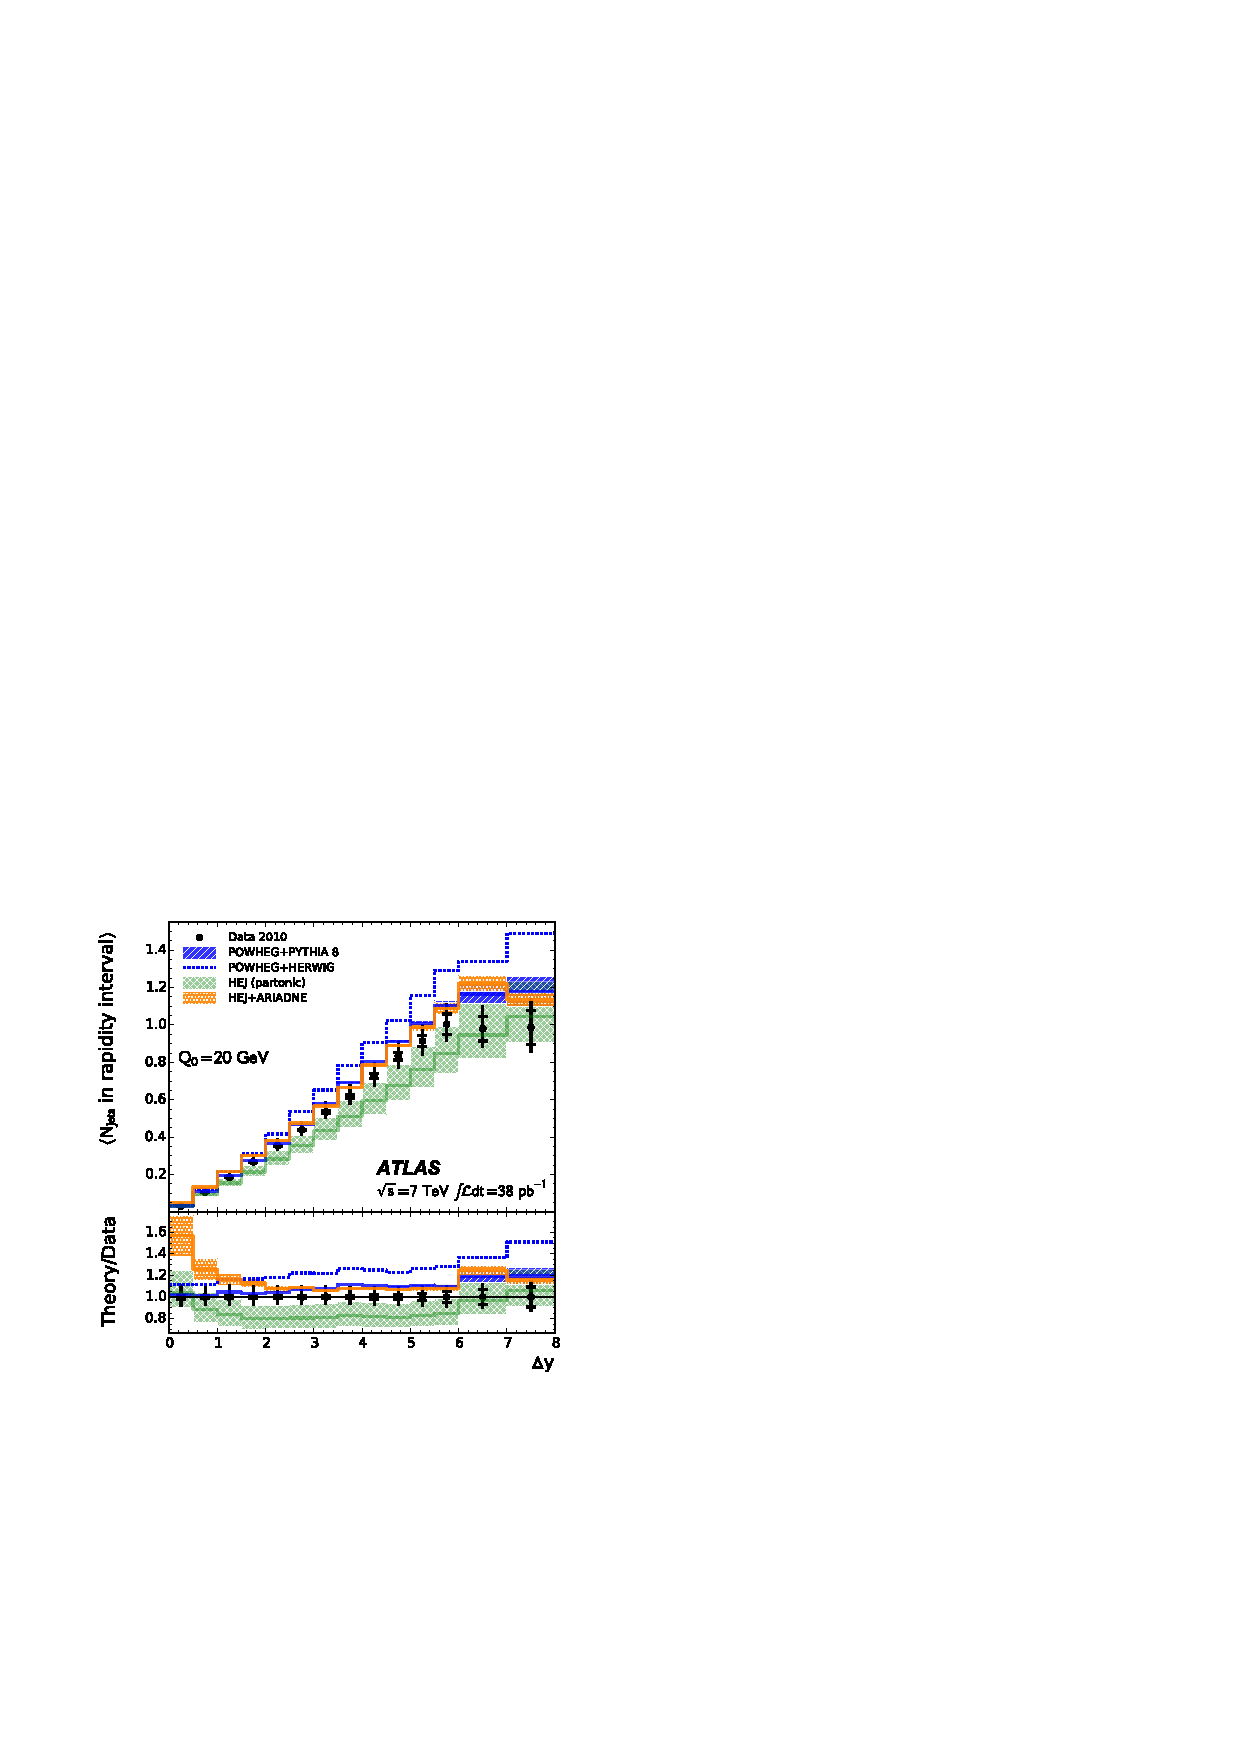
\includegraphics[width=\textwidth, height=1.0\textwidth]{pureJets4a}
			\caption{}
			\label{fig:}
		\end{subfigure}
		~
		\begin{subfigure}[b]{0.48\textwidth}
			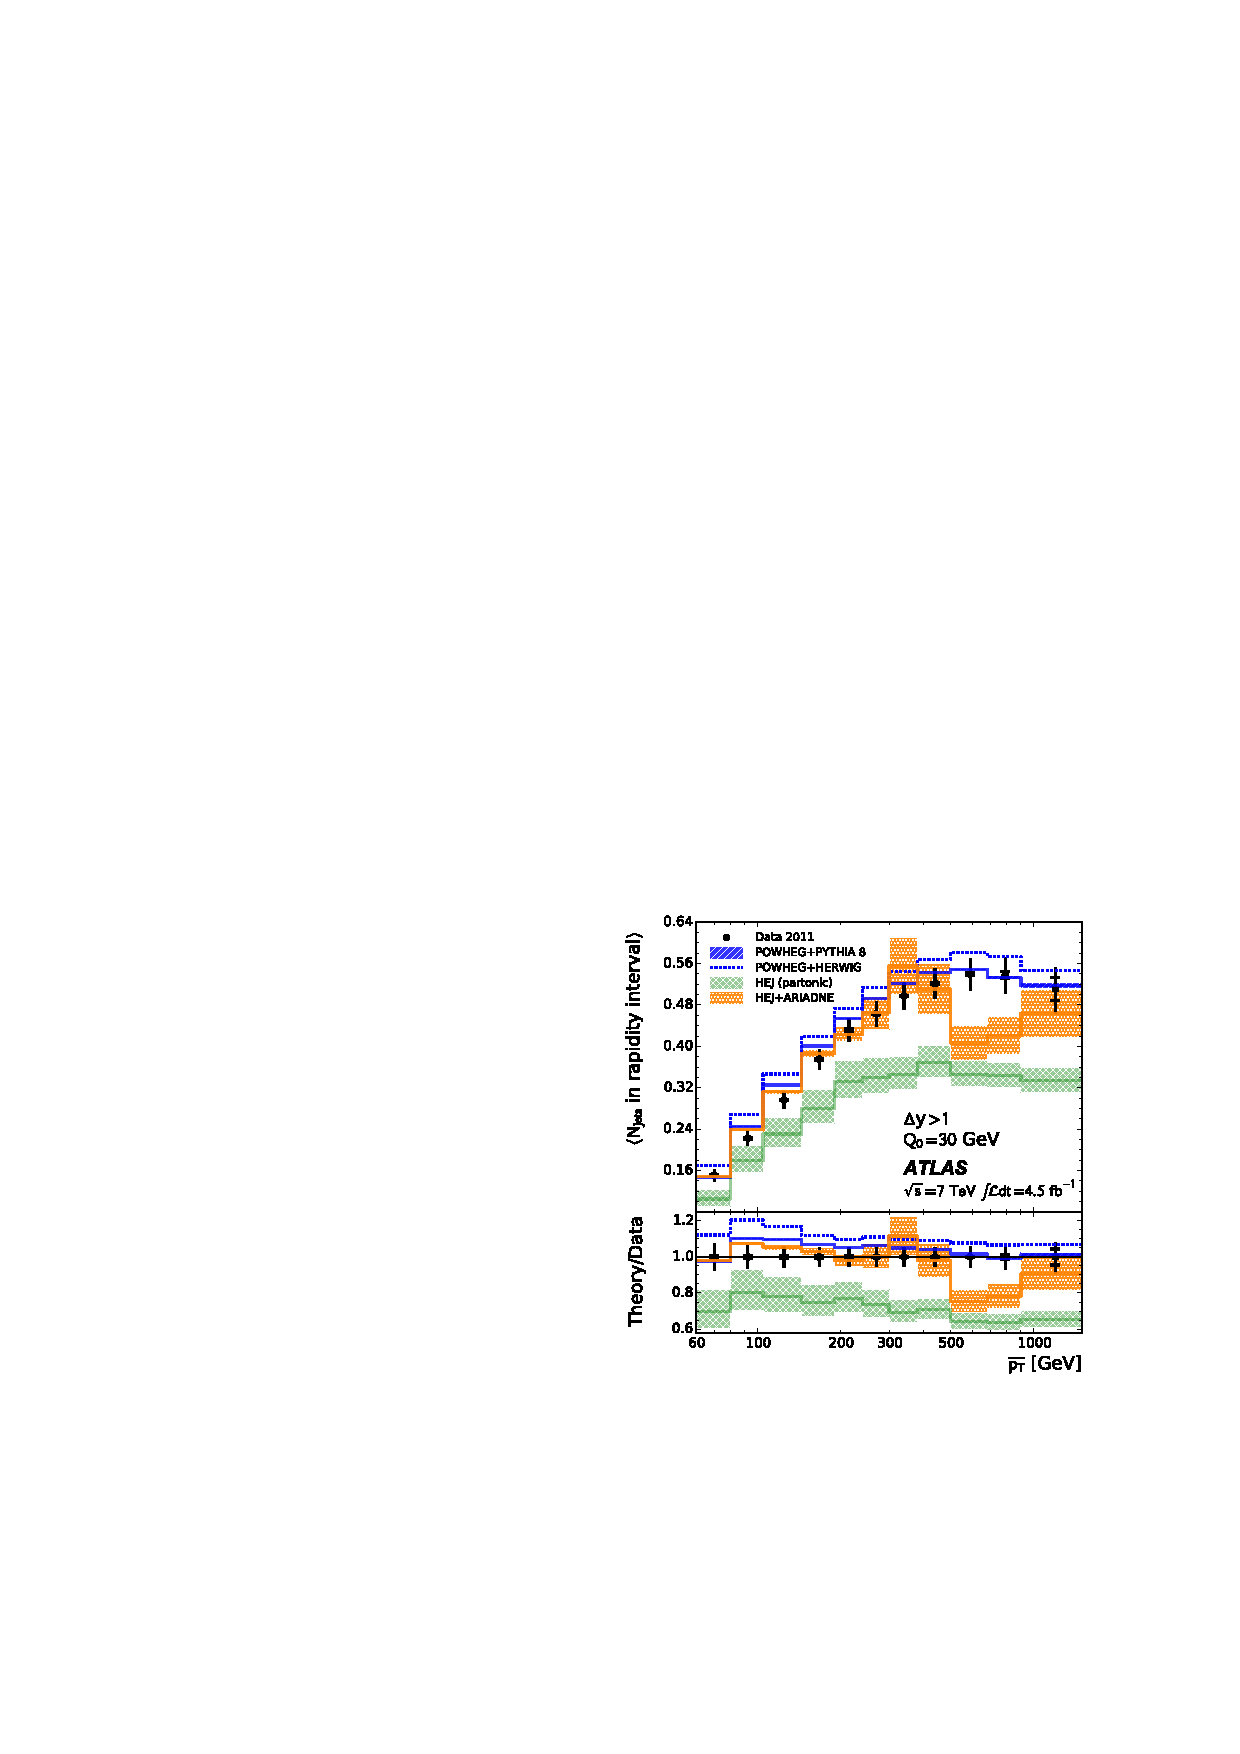
\includegraphics[width=\textwidth, height=1.0\textwidth]{pureJets4b}
			\caption{}
			\label{fig:}
		\end{subfigure}
		\caption{}
		\label{fig:}
	\end{figure}

	\begin{figure}[H]
		\centering
		\begin{subfigure}[b]{0.48\textwidth}
			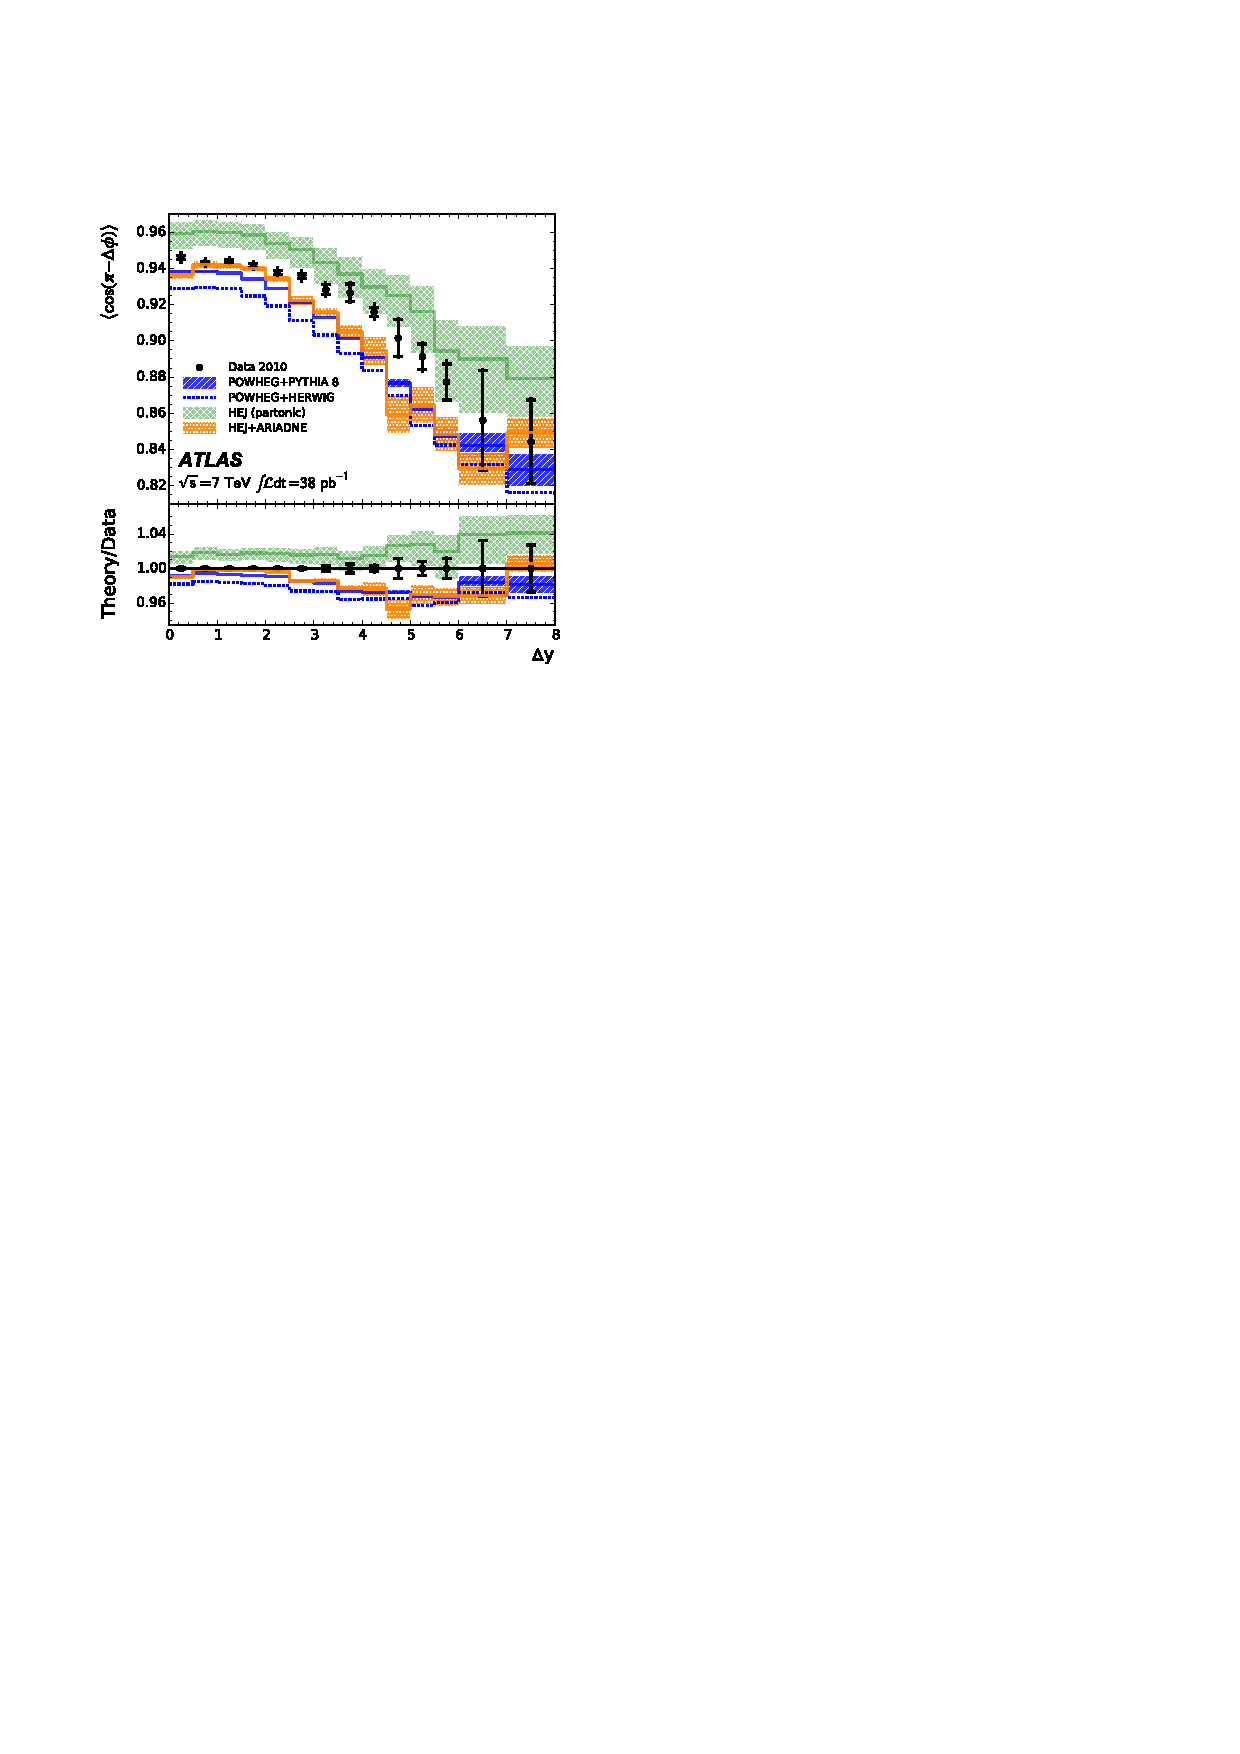
\includegraphics[width=\textwidth, height=1.0\textwidth]{pureJets5a}
			\caption{}
			\label{fig:}
		\end{subfigure}
		~
		\begin{subfigure}[b]{0.48\textwidth}
			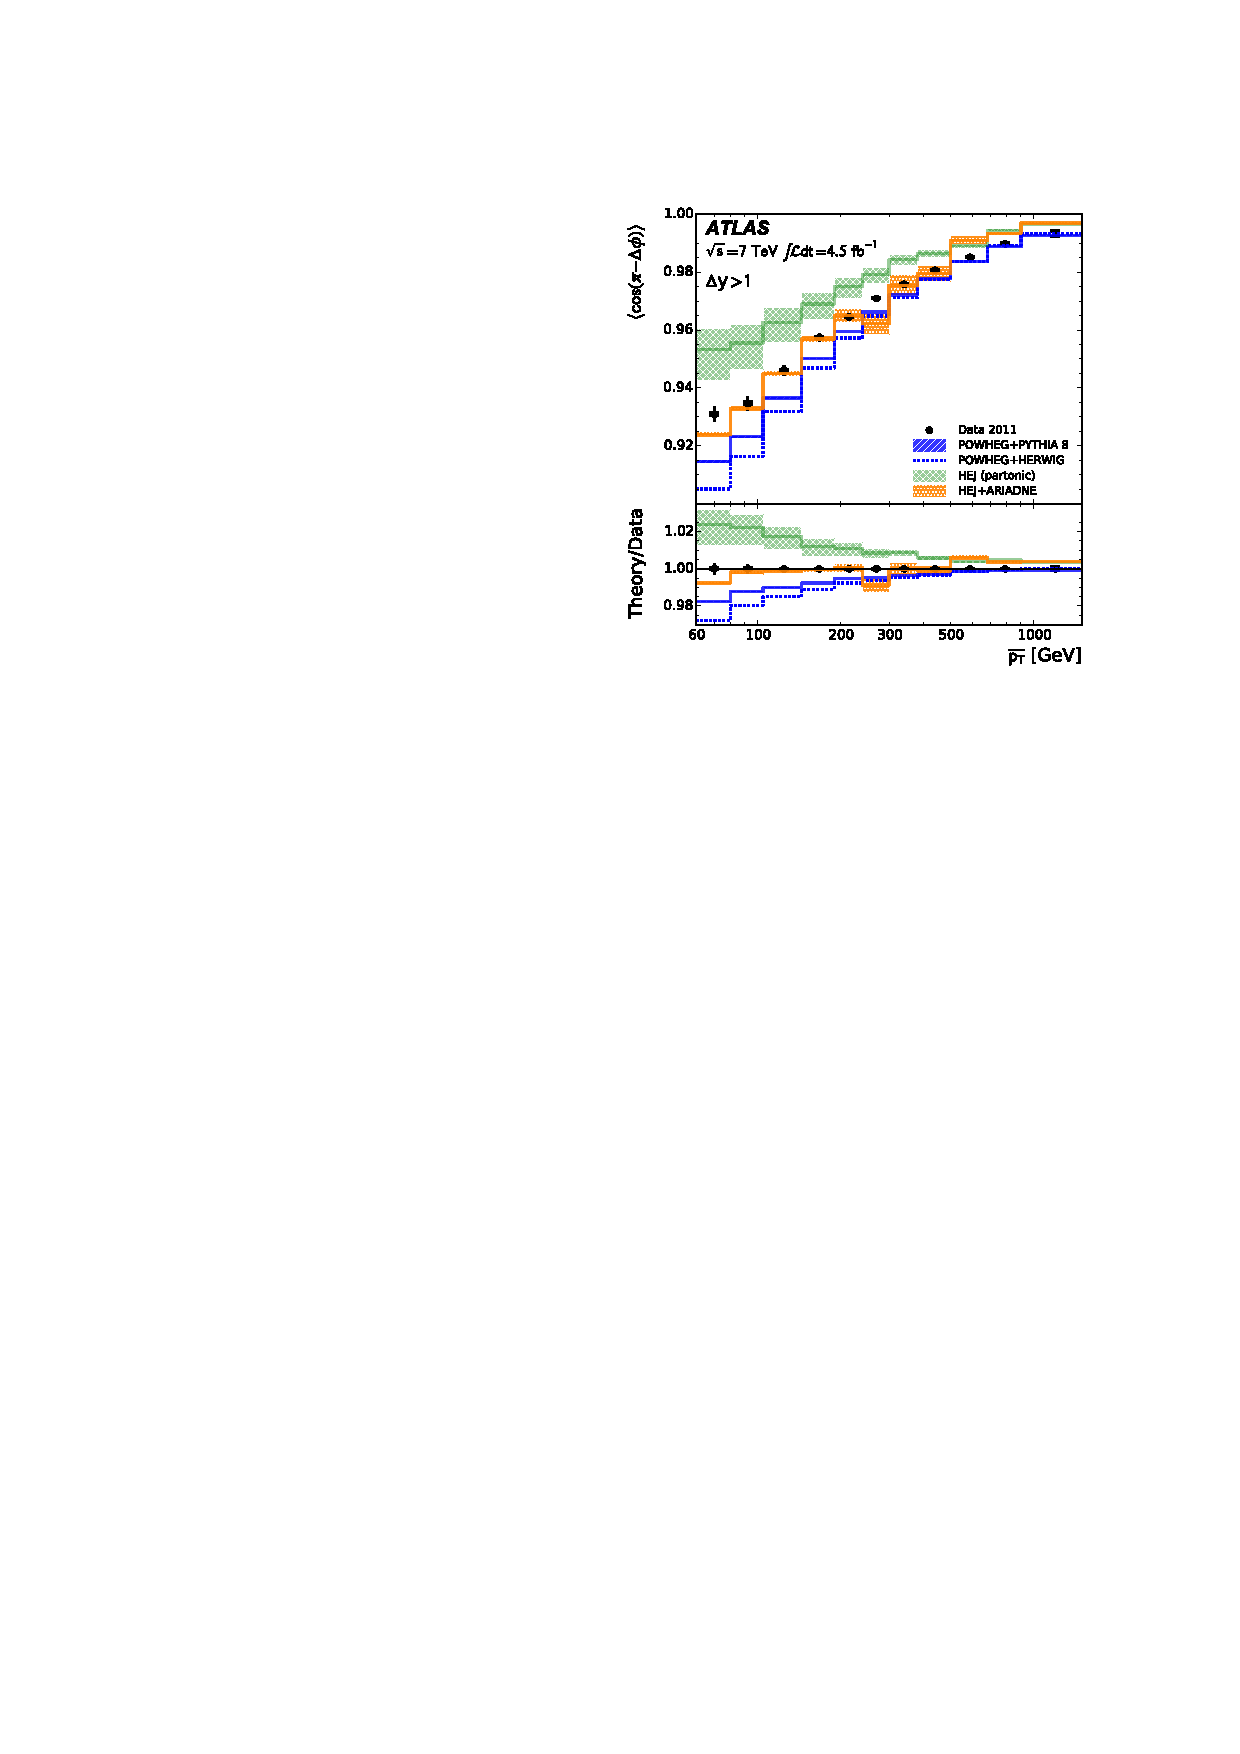
\includegraphics[width=\textwidth, height=1.0\textwidth]{pureJets5b}
			\caption{}
			\label{fig:}
		\end{subfigure}
		\caption{}
		\label{fig:}

		\begin{subfigure}[b]{0.48\textwidth}
			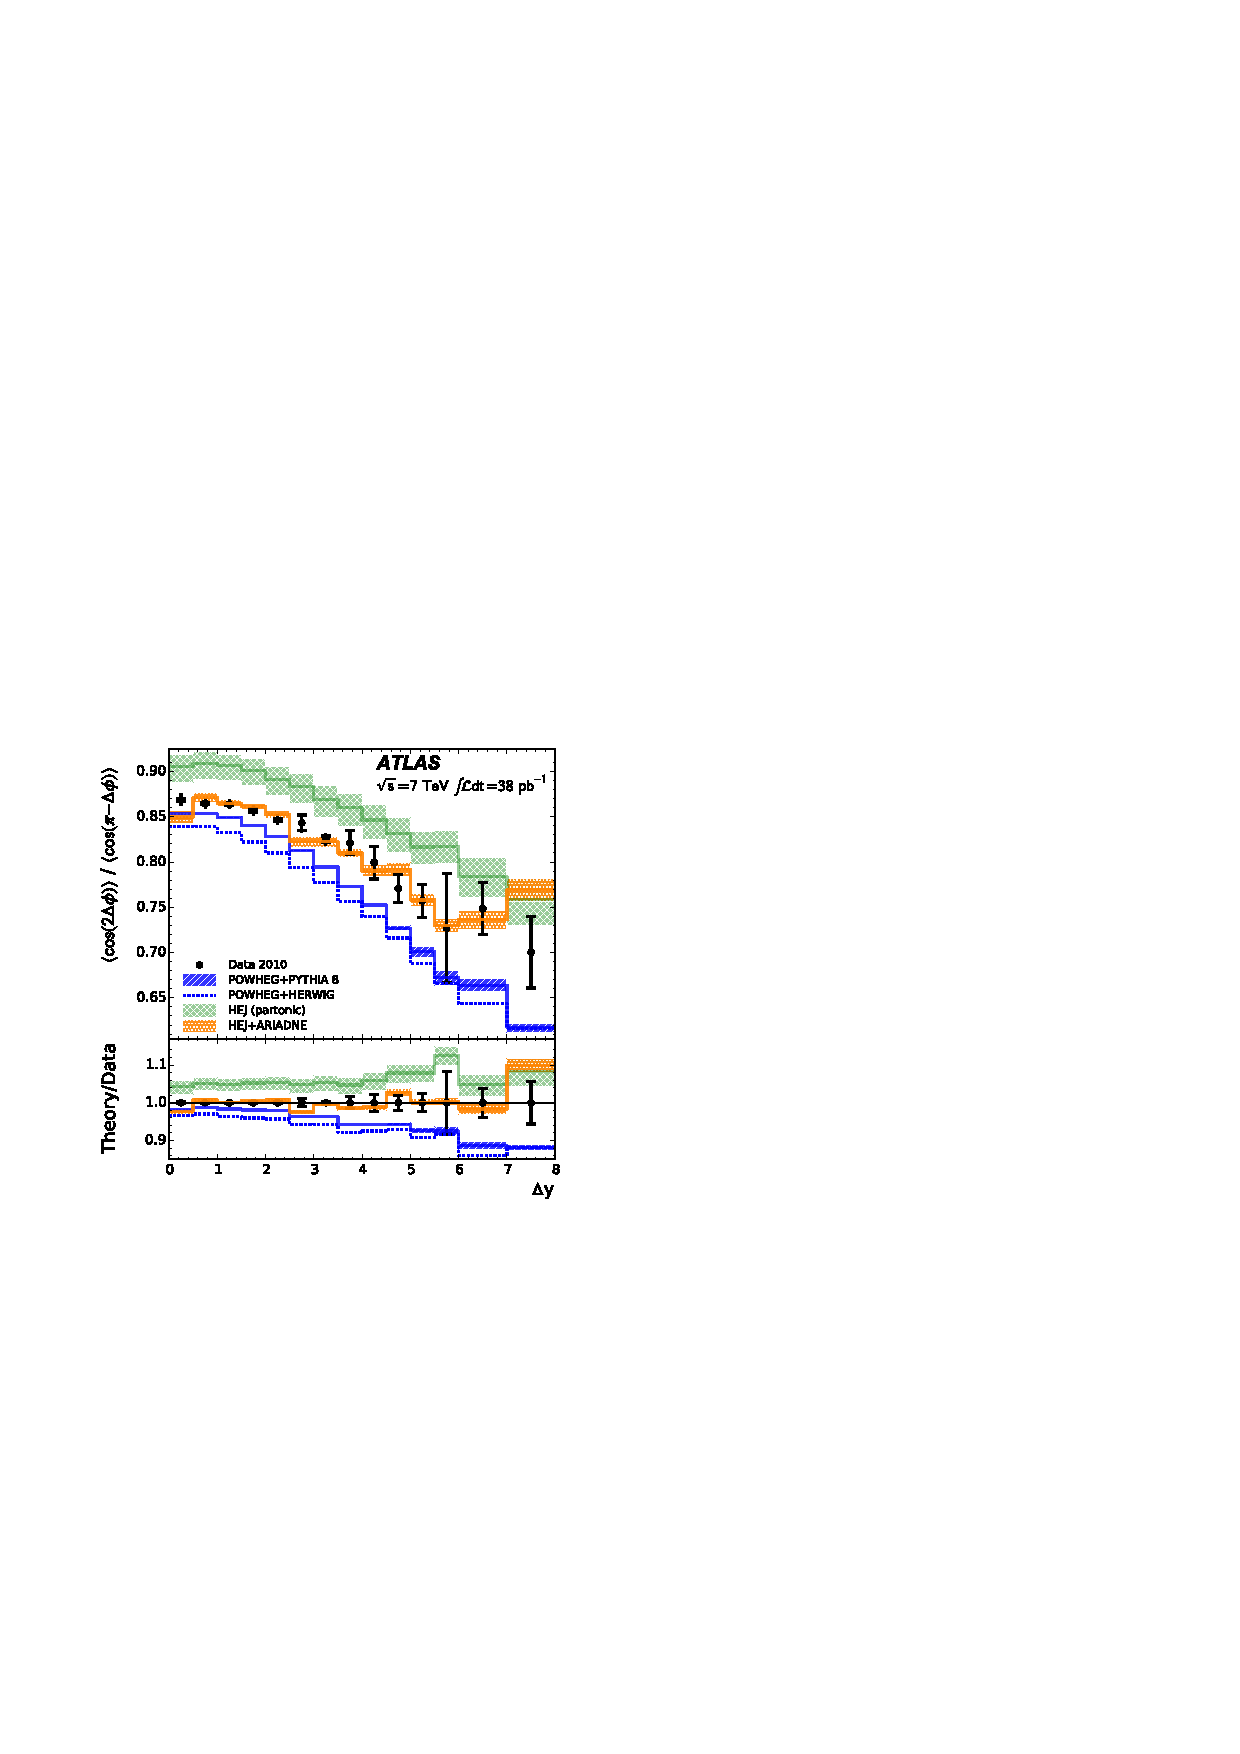
\includegraphics[width=\textwidth, height=1.0\textwidth]{pureJets5c}
			\caption{}
			\label{fig:}
		\end{subfigure}
		~
		\begin{subfigure}[b]{0.48\textwidth}
			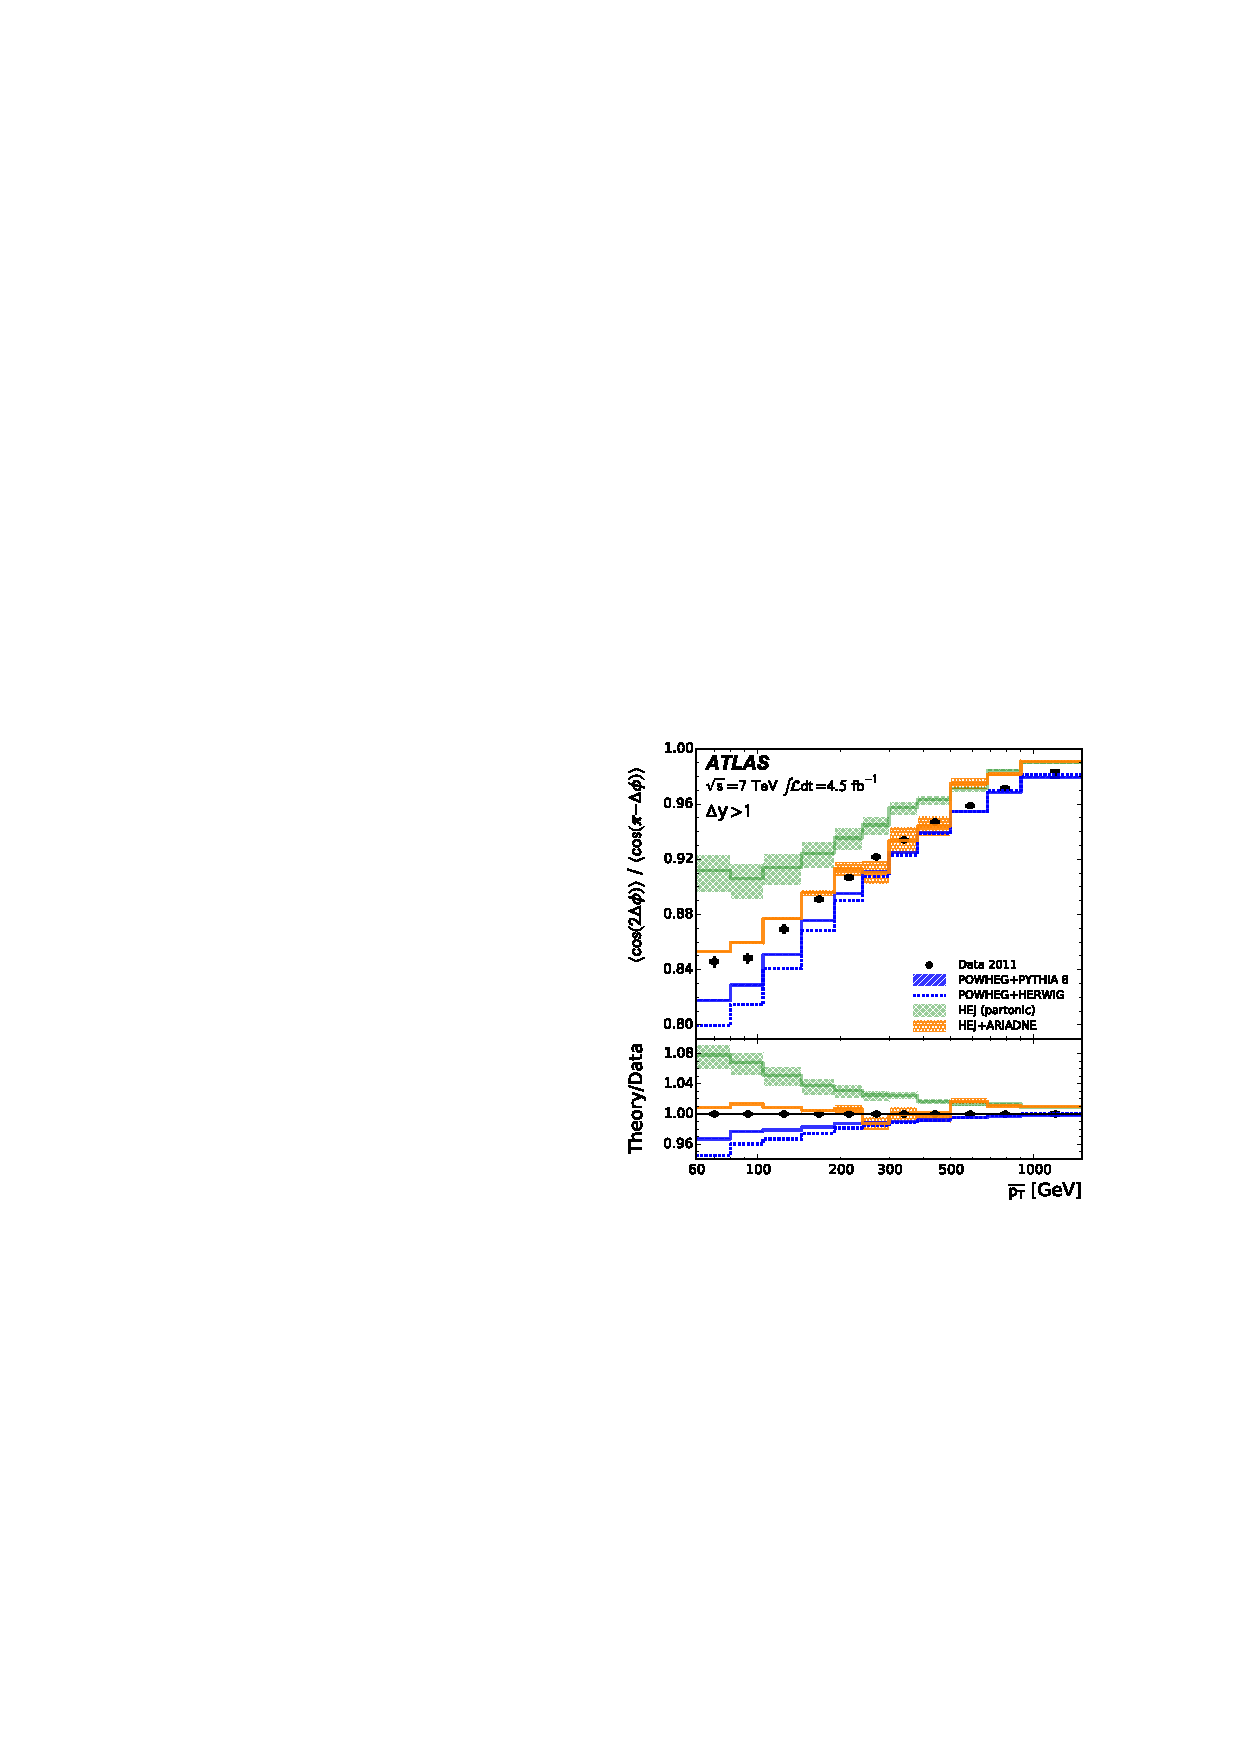
\includegraphics[width=\textwidth, height=1.0\textwidth]{pureJets5d}
			\caption{}
			\label{fig:}
		\end{subfigure}
		\caption{}
		\label{fig:}
	\end{figure}

	\begin{figure}[H]
		\centering
		\begin{subfigure}[b]{0.48\textwidth}
			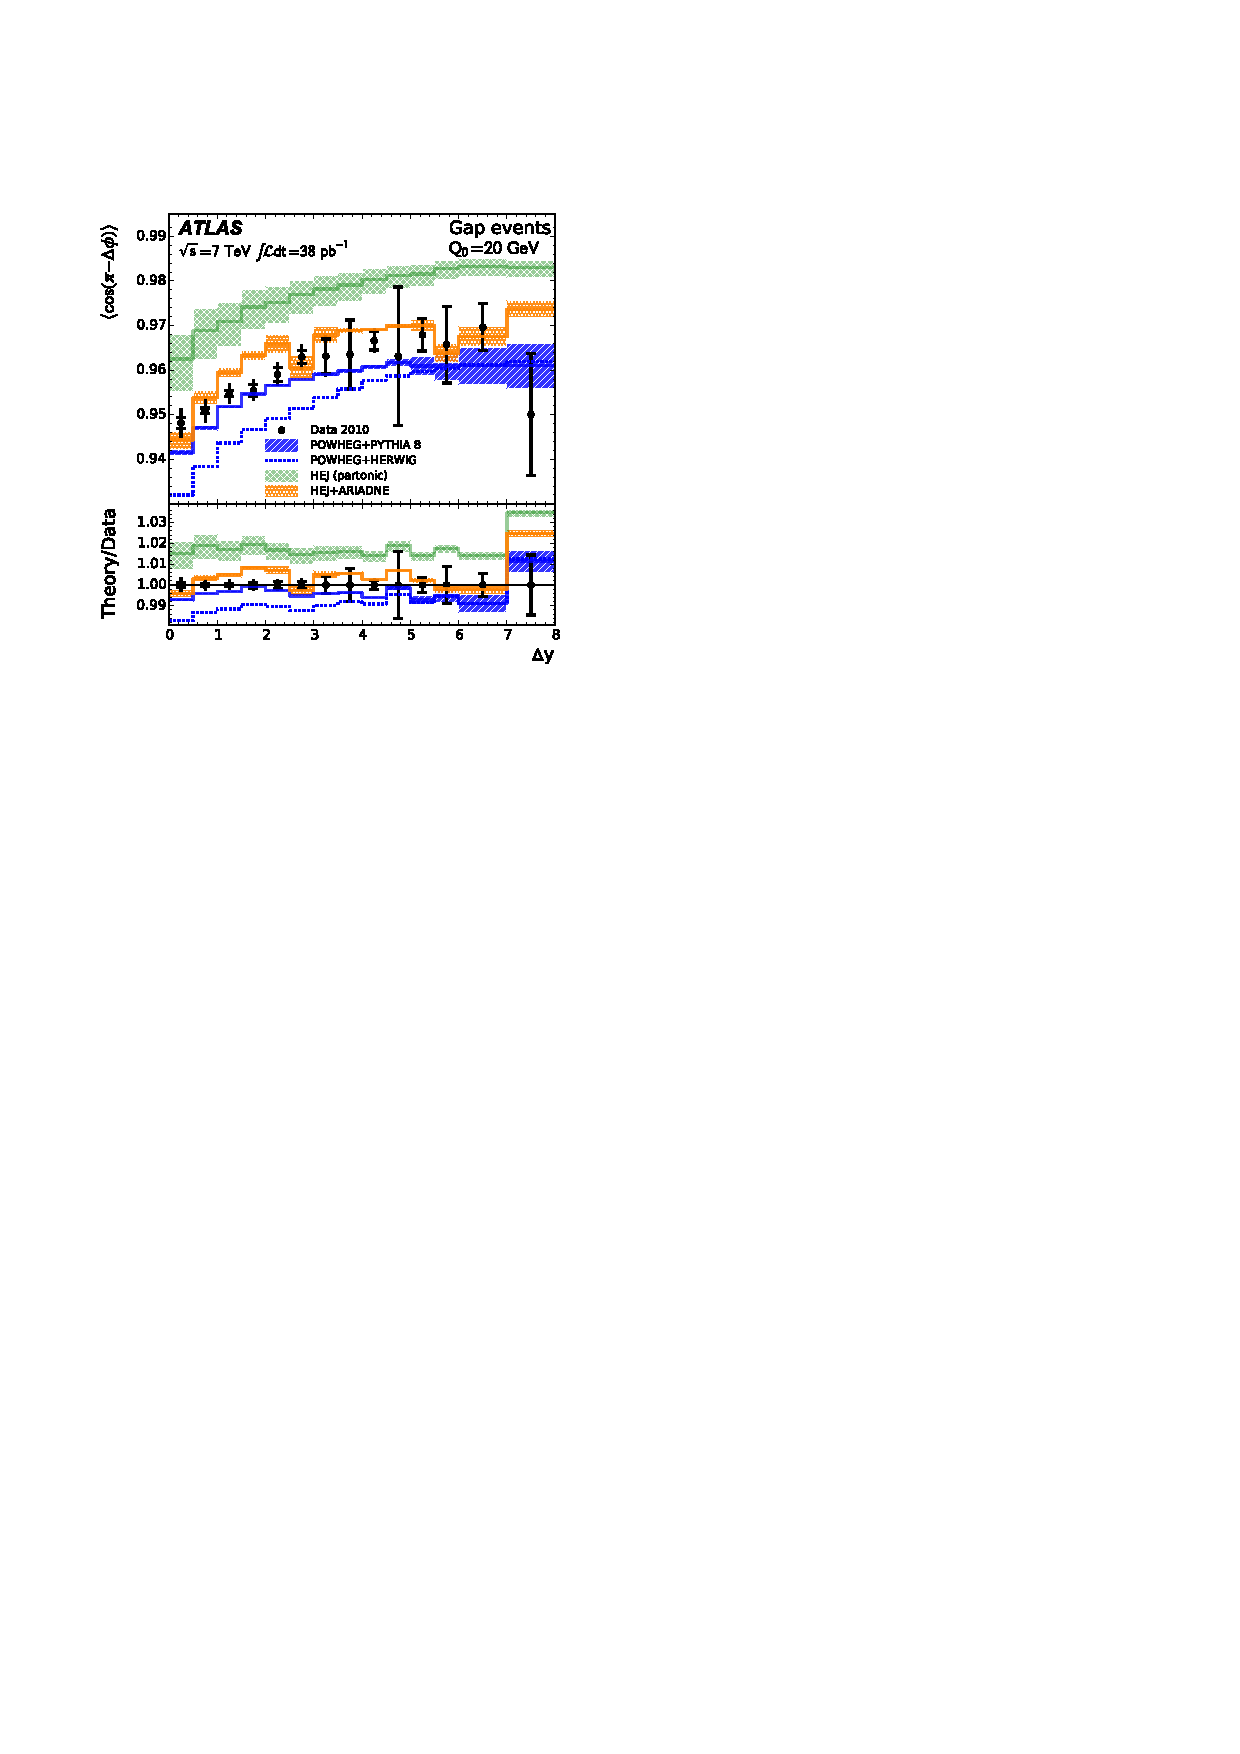
\includegraphics[width=\textwidth, height=1.0\textwidth]{pureJets6a}
			\caption{}
			\label{fig:}
		\end{subfigure}
		~
		\begin{subfigure}[b]{0.48\textwidth}
			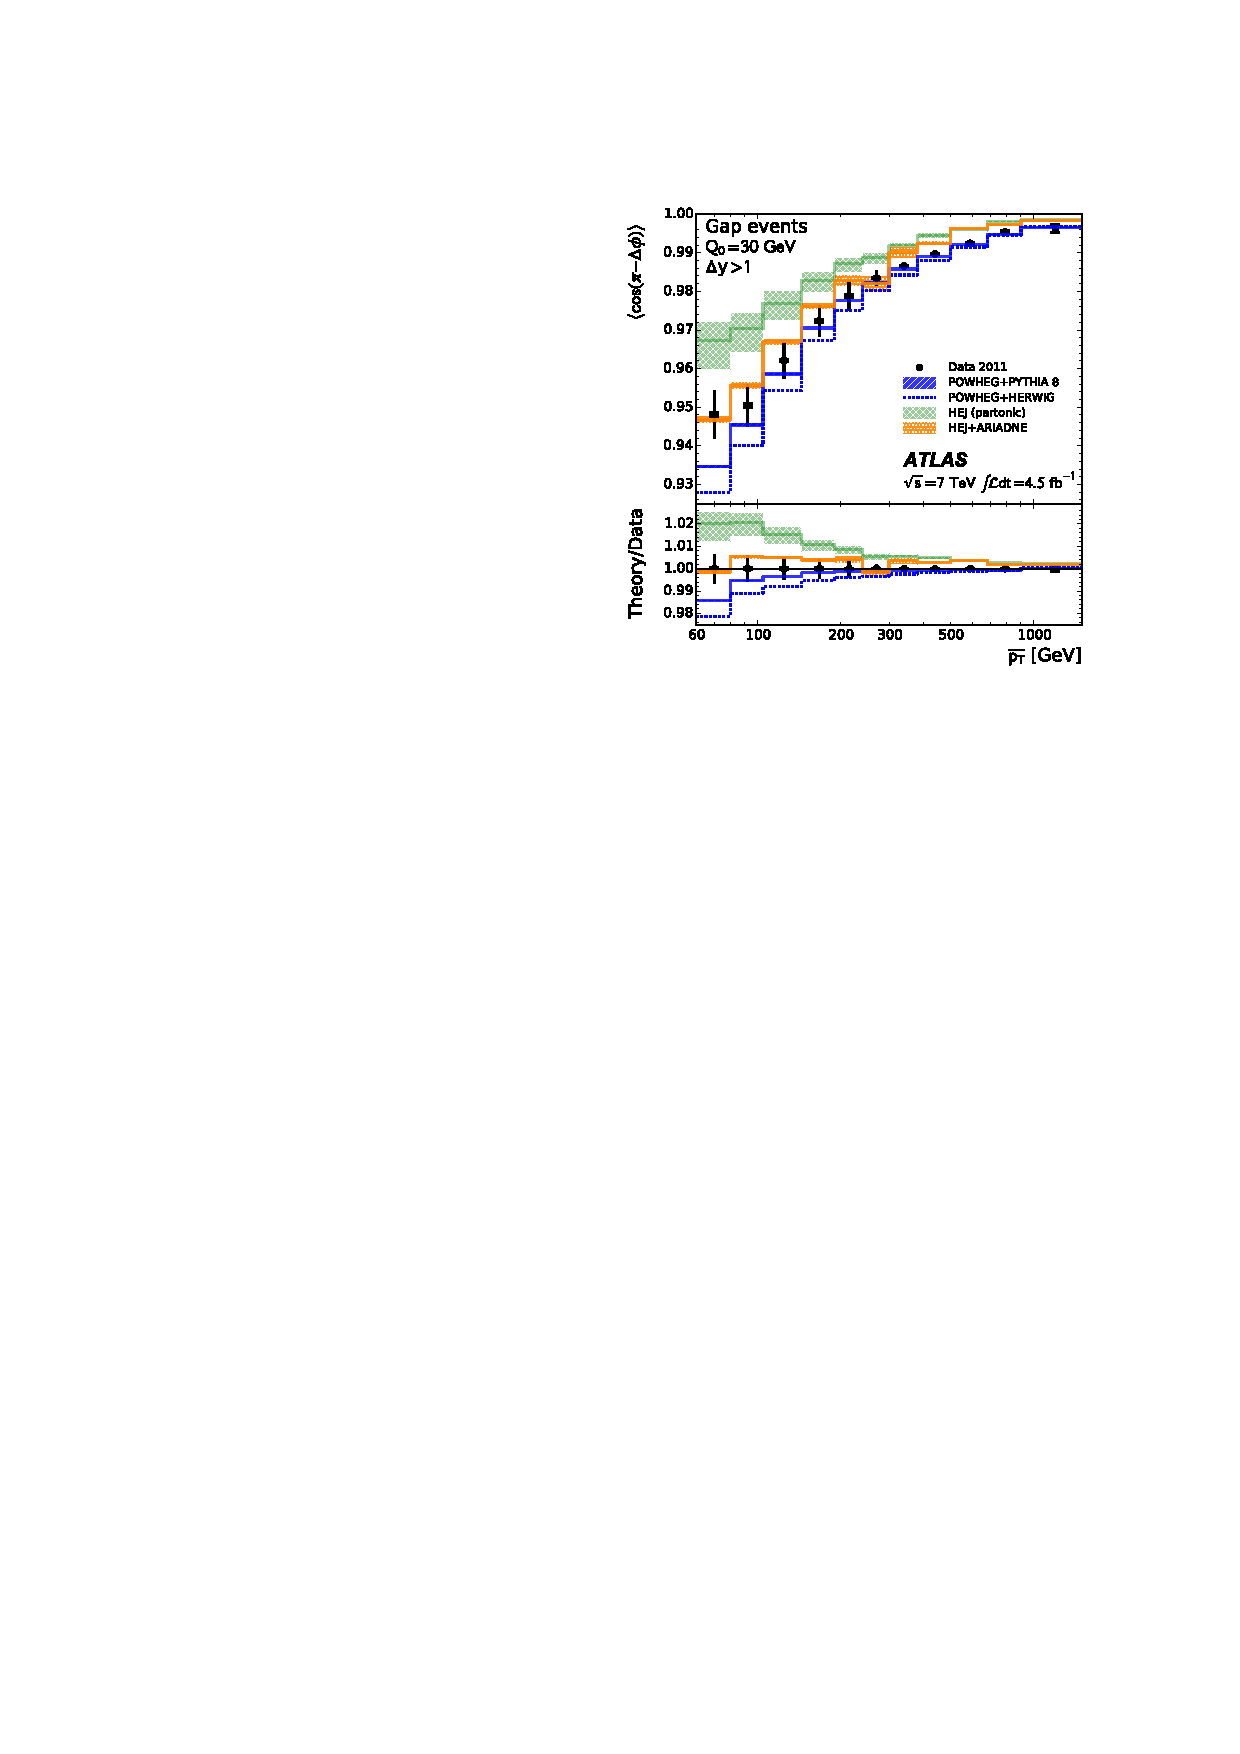
\includegraphics[width=\textwidth, height=1.0\textwidth]{pureJets6b}
			\caption{}
			\label{fig:}
		\end{subfigure}
		\caption{}
		\label{fig:}

		\begin{subfigure}[b]{0.48\textwidth}
			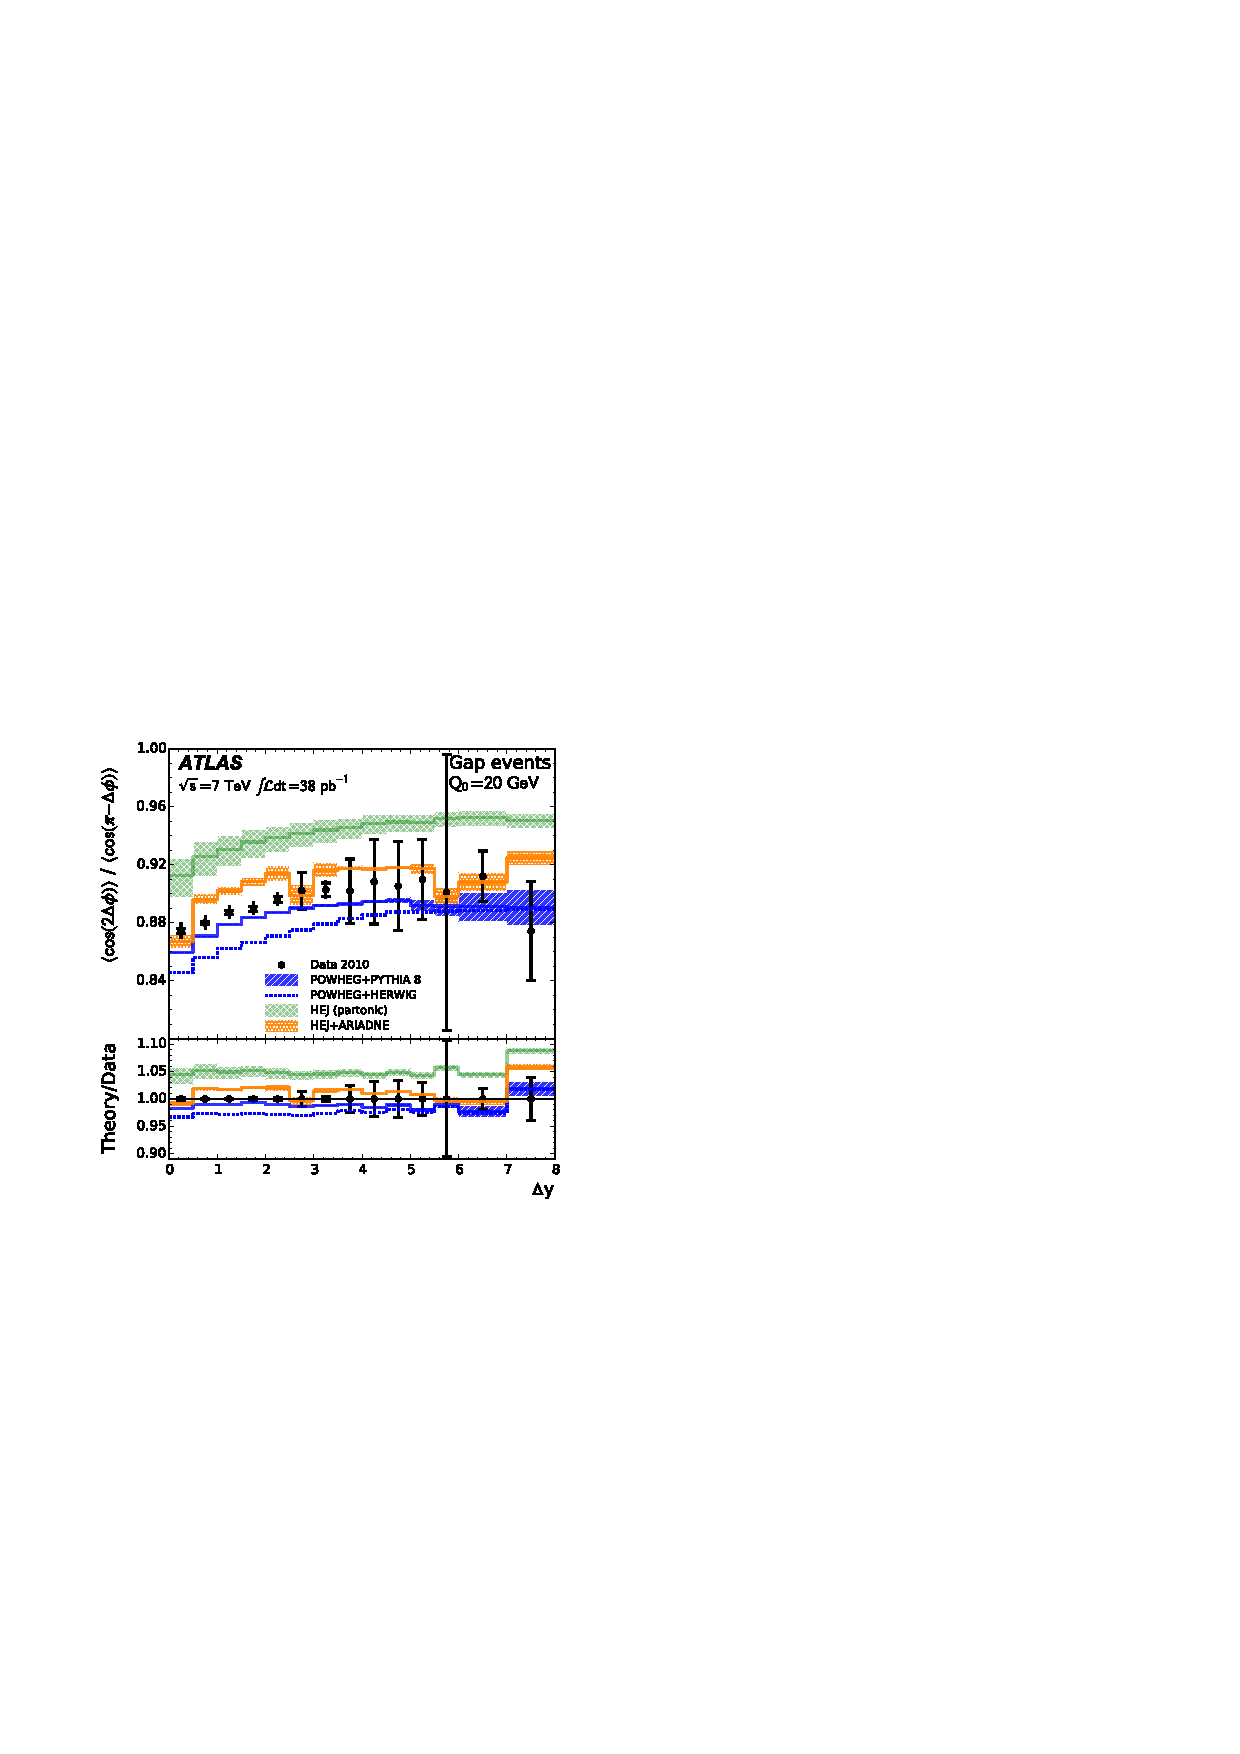
\includegraphics[width=\textwidth, height=1.0\textwidth]{pureJets6c}
			\caption{}
			\label{fig:}
		\end{subfigure}
		~
		\begin{subfigure}[b]{0.48\textwidth}
			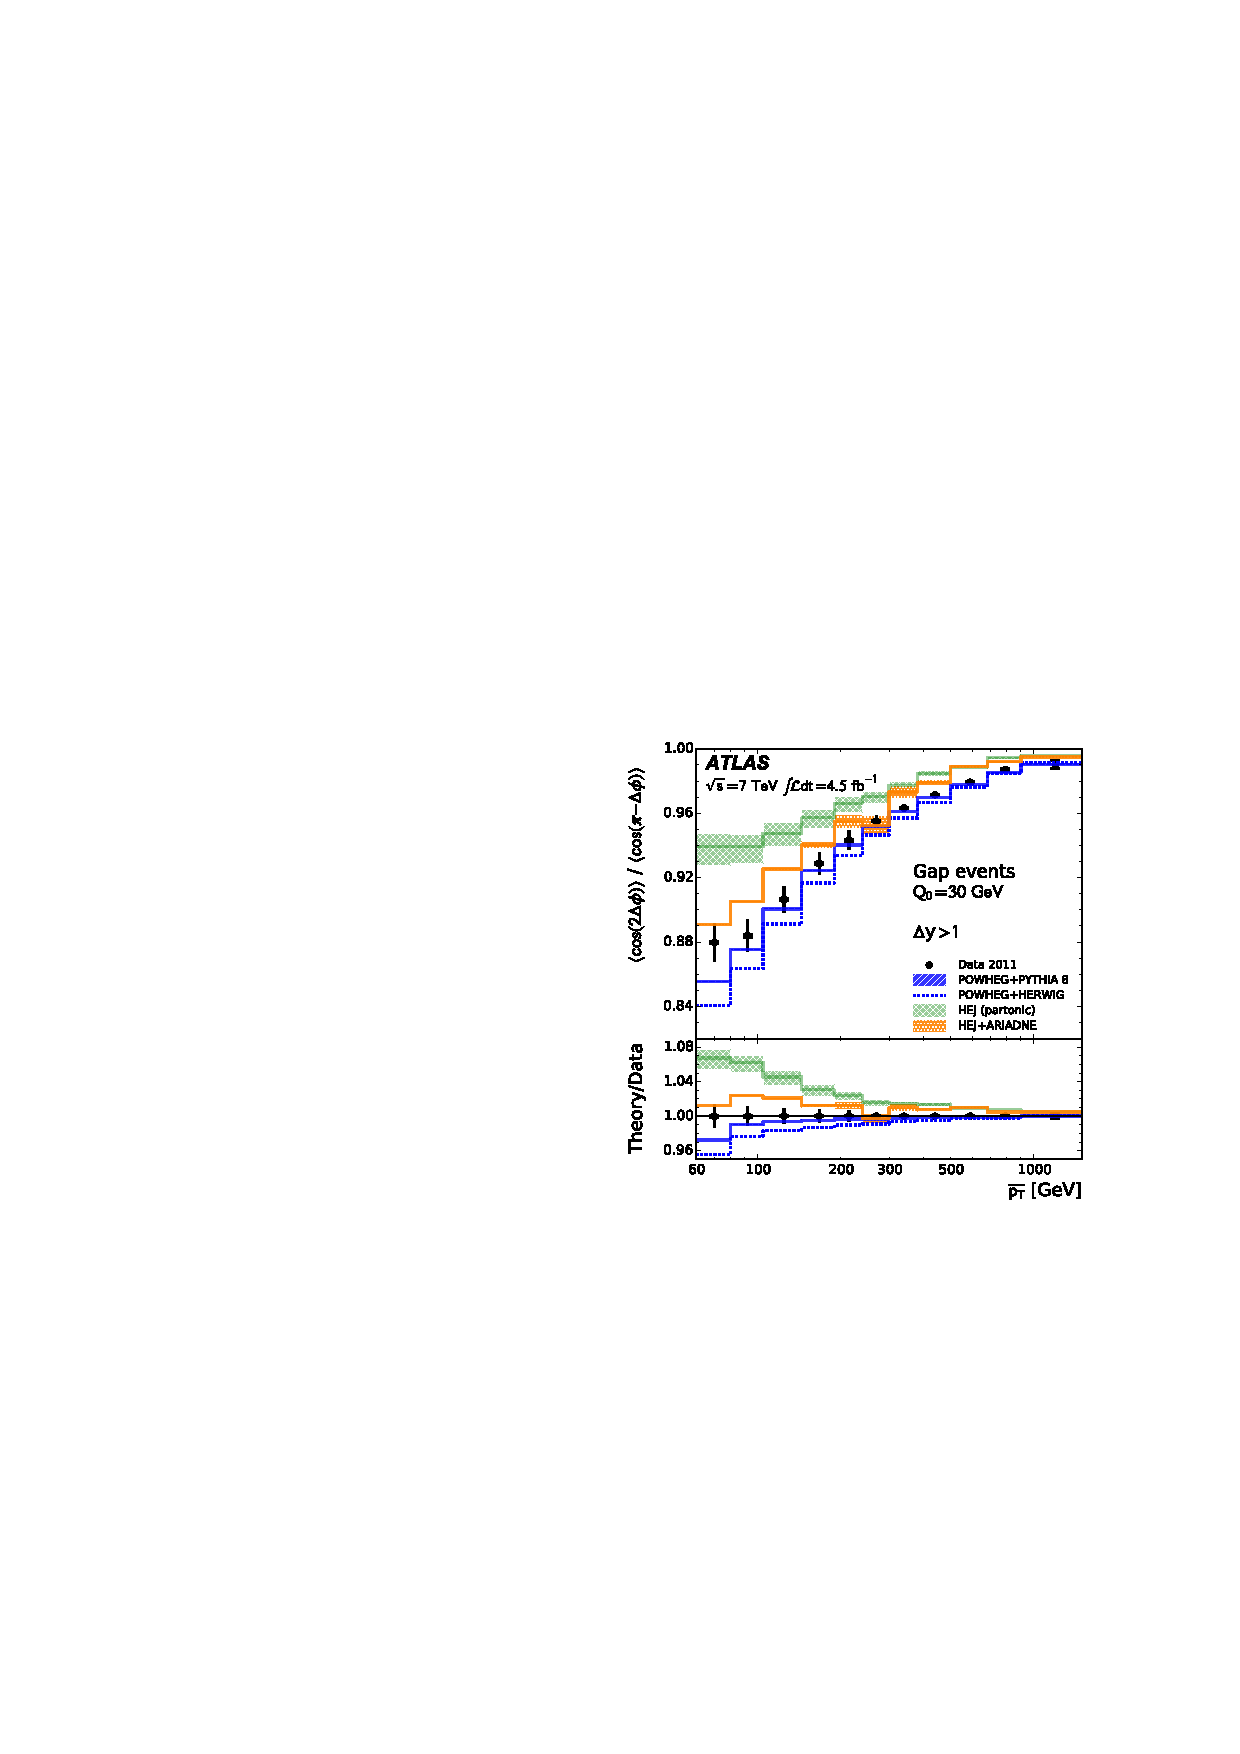
\includegraphics[width=\textwidth, height=1.0\textwidth]{pureJets6d}
			\caption{}
			\label{fig:}
		\end{subfigure}
		\caption{}
		\label{fig:}
	\end{figure}

	\begin{figure}[H]
		\centering
		\begin{subfigure}[b]{0.48\textwidth}
			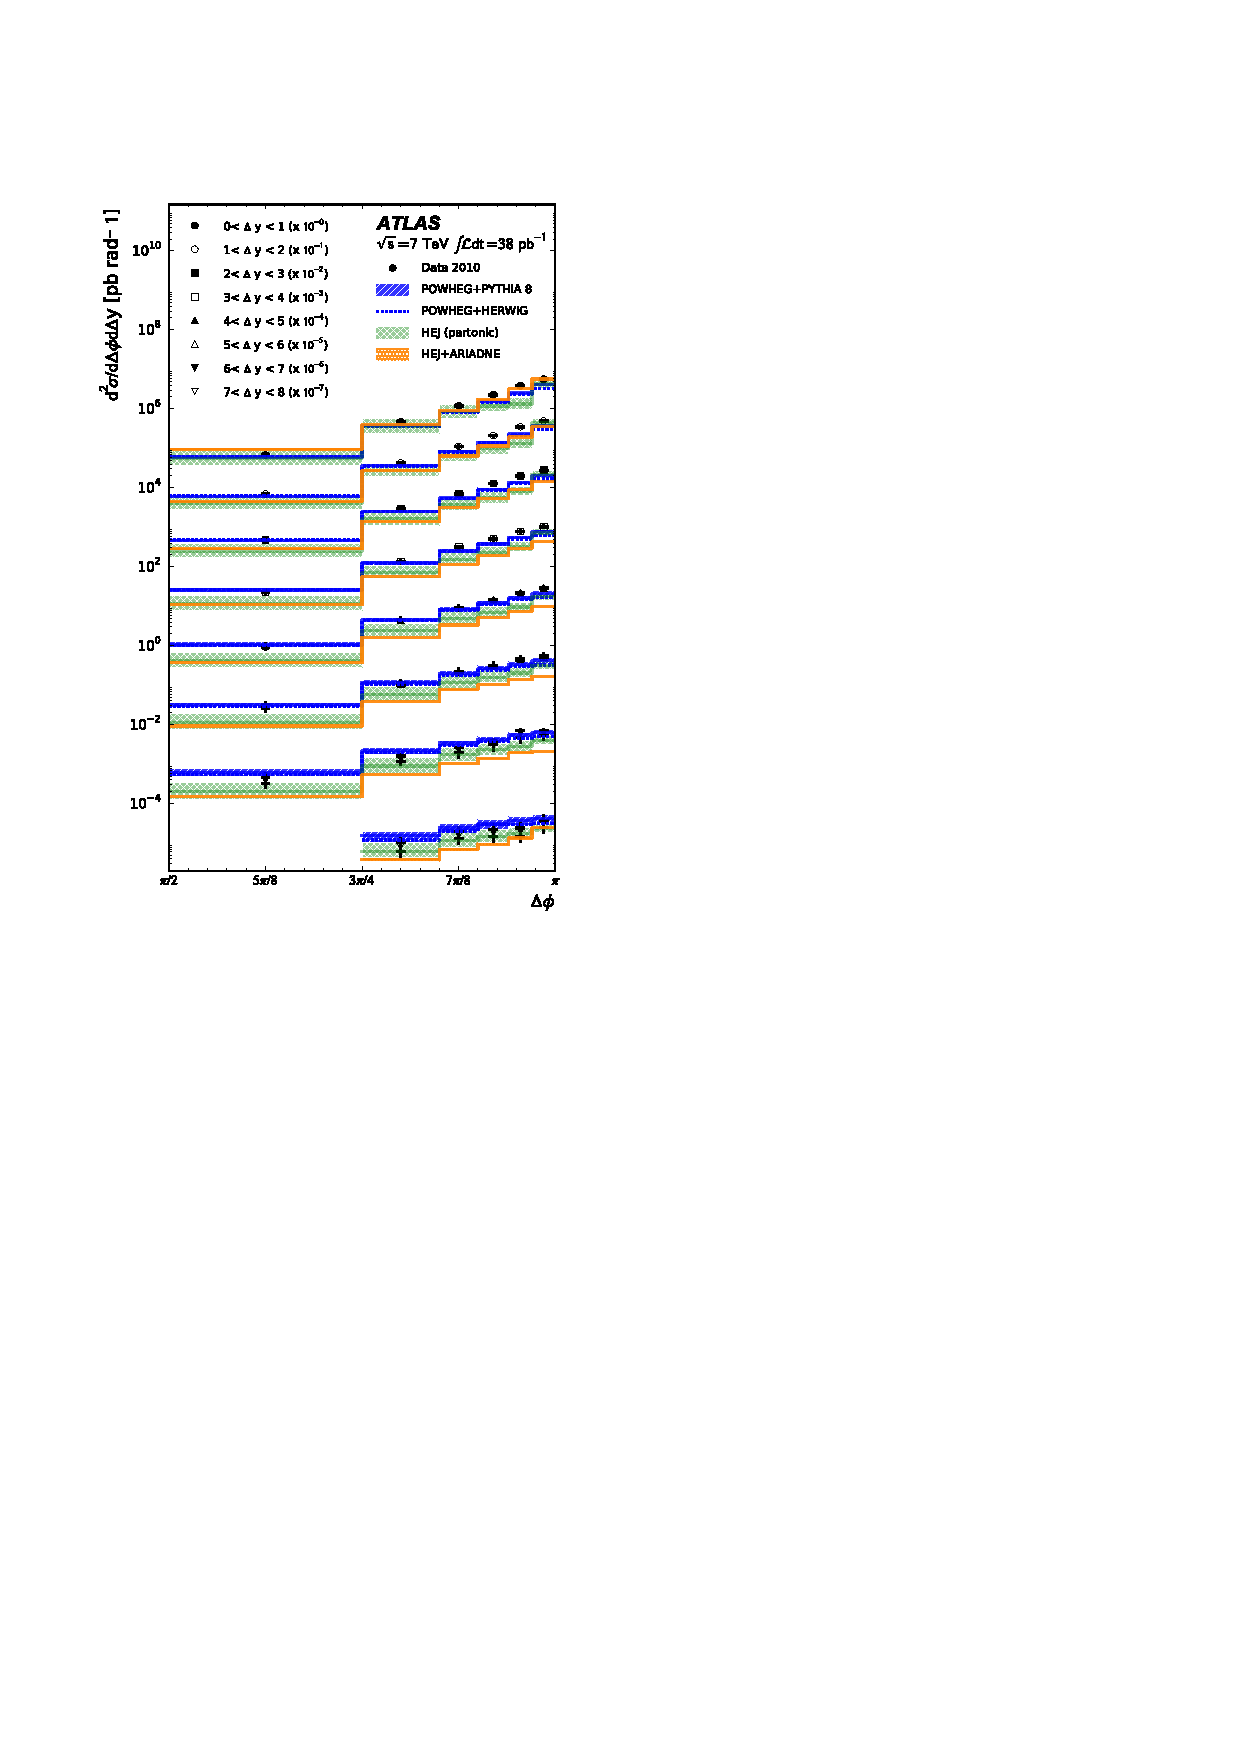
\includegraphics[width=\textwidth, height=1.0\textwidth]{pureJets7a}
			\caption{}
			\label{fig:}
		\end{subfigure}
		~
		\begin{subfigure}[b]{0.48\textwidth}
			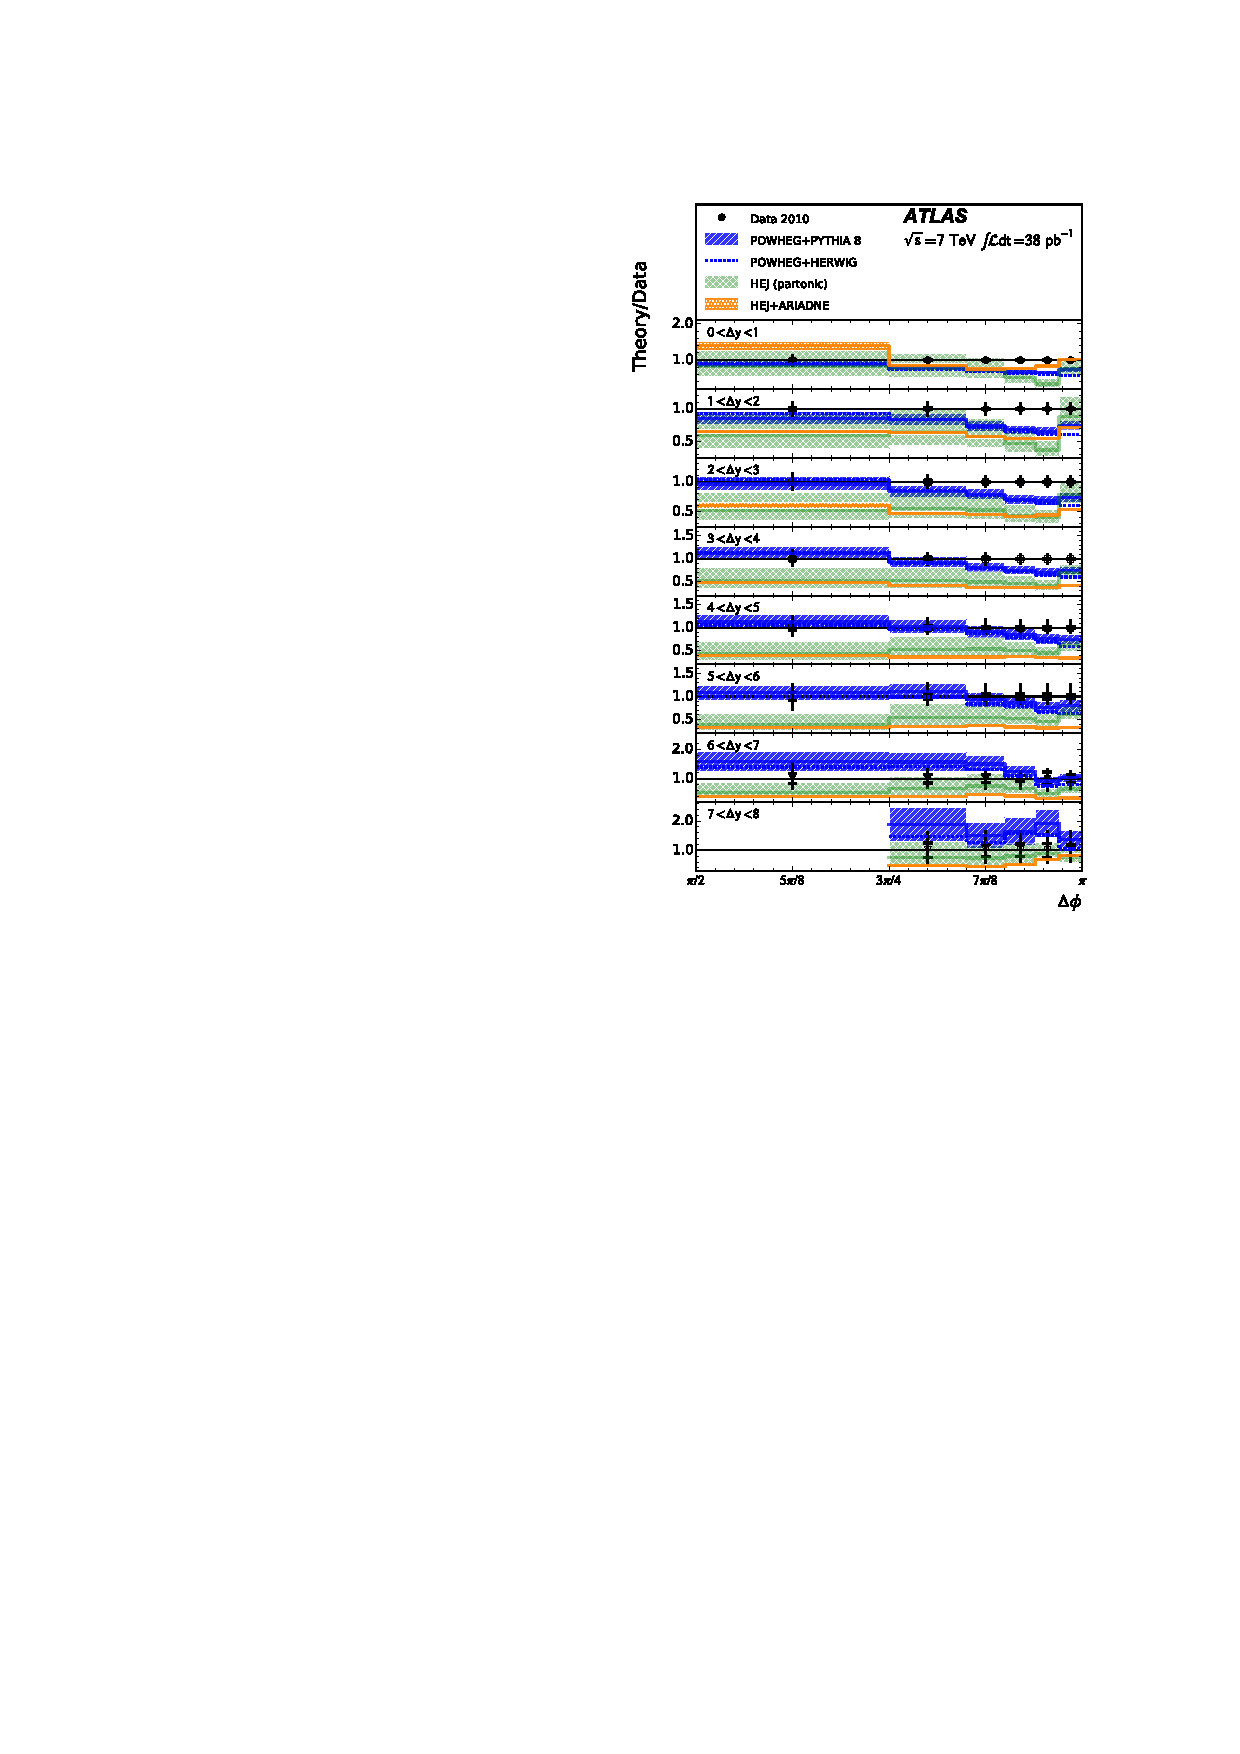
\includegraphics[width=\textwidth, height=1.0\textwidth]{pureJets7b}
			\caption{}
			\label{fig:}
		\end{subfigure}
		\caption{}
		\label{fig:}

		\begin{subfigure}[b]{0.48\textwidth}
			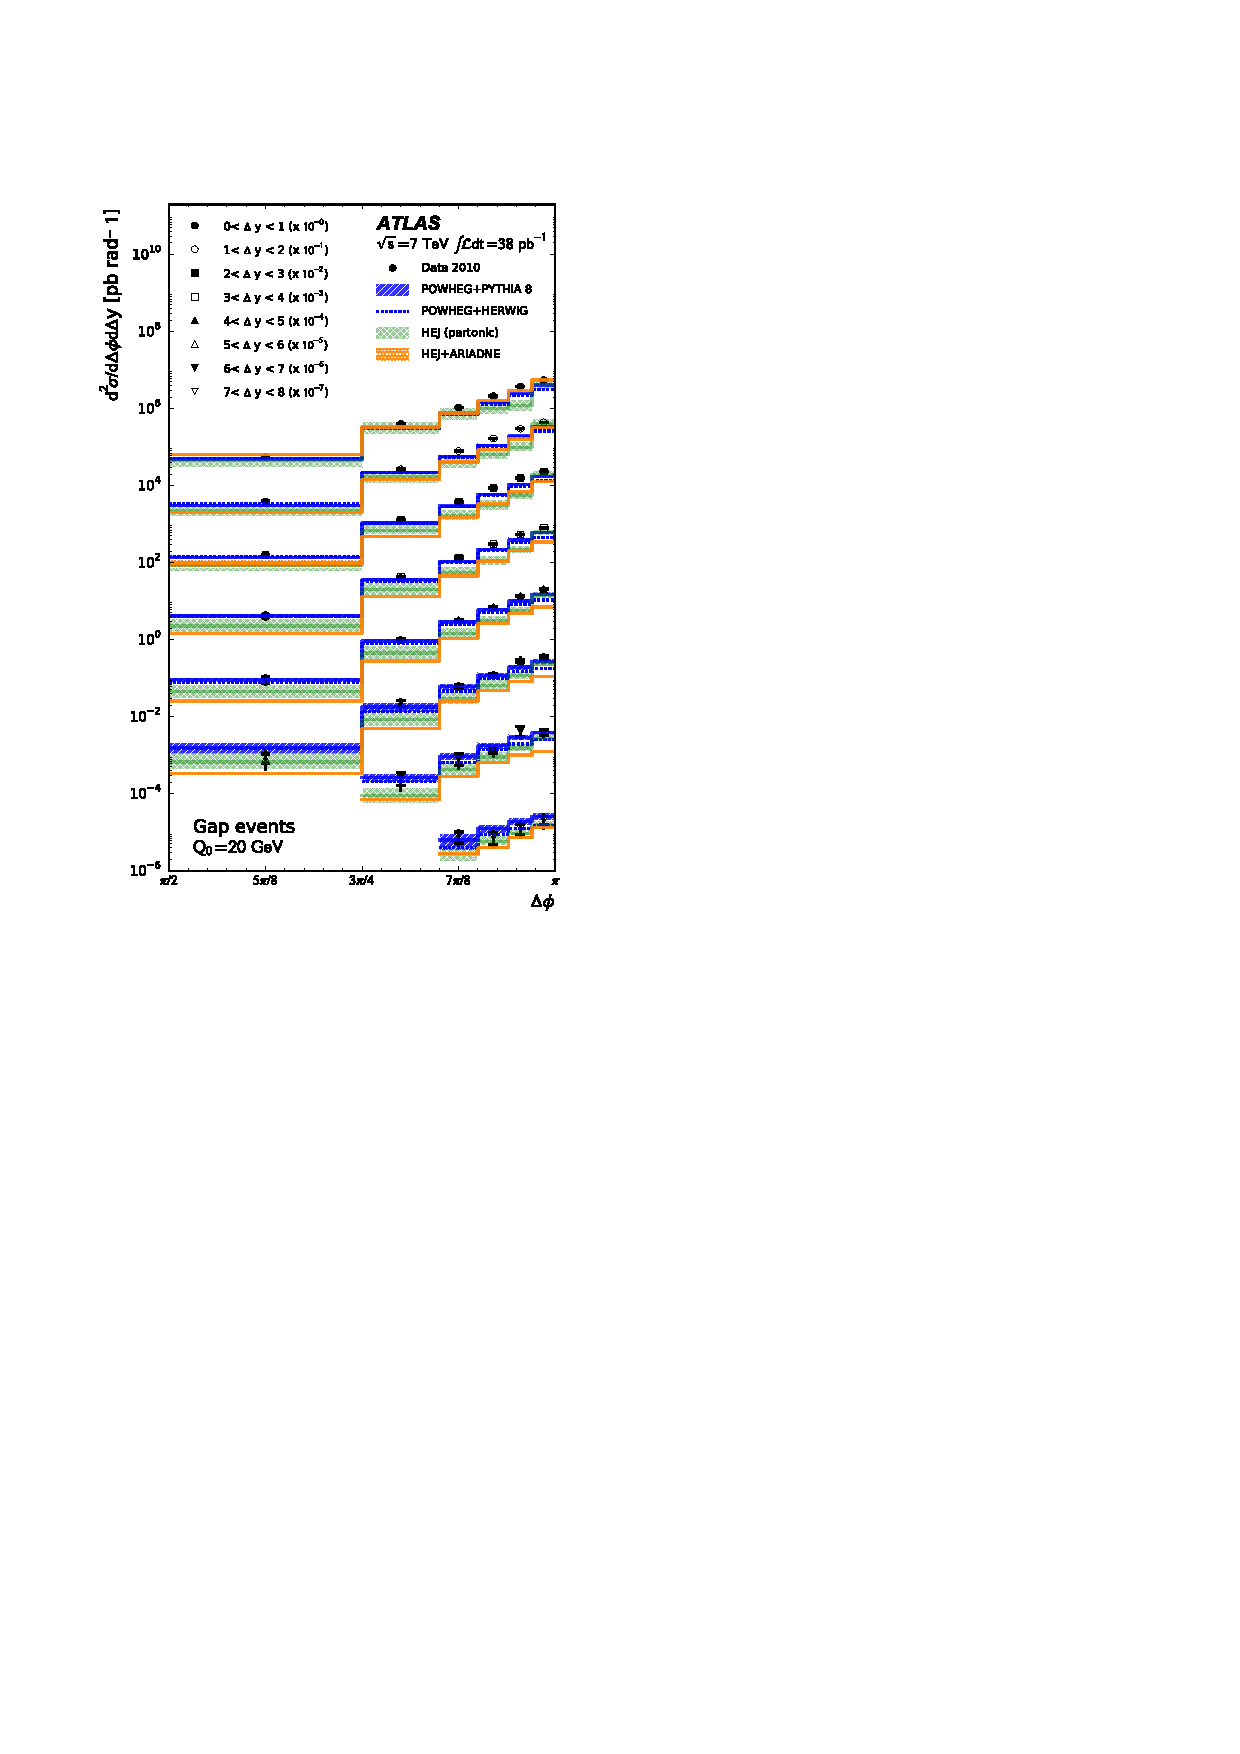
\includegraphics[width=\textwidth, height=1.0\textwidth]{pureJets8a}
			\caption{}
			\label{fig:}
		\end{subfigure}
		~
		\begin{subfigure}[b]{0.48\textwidth}
			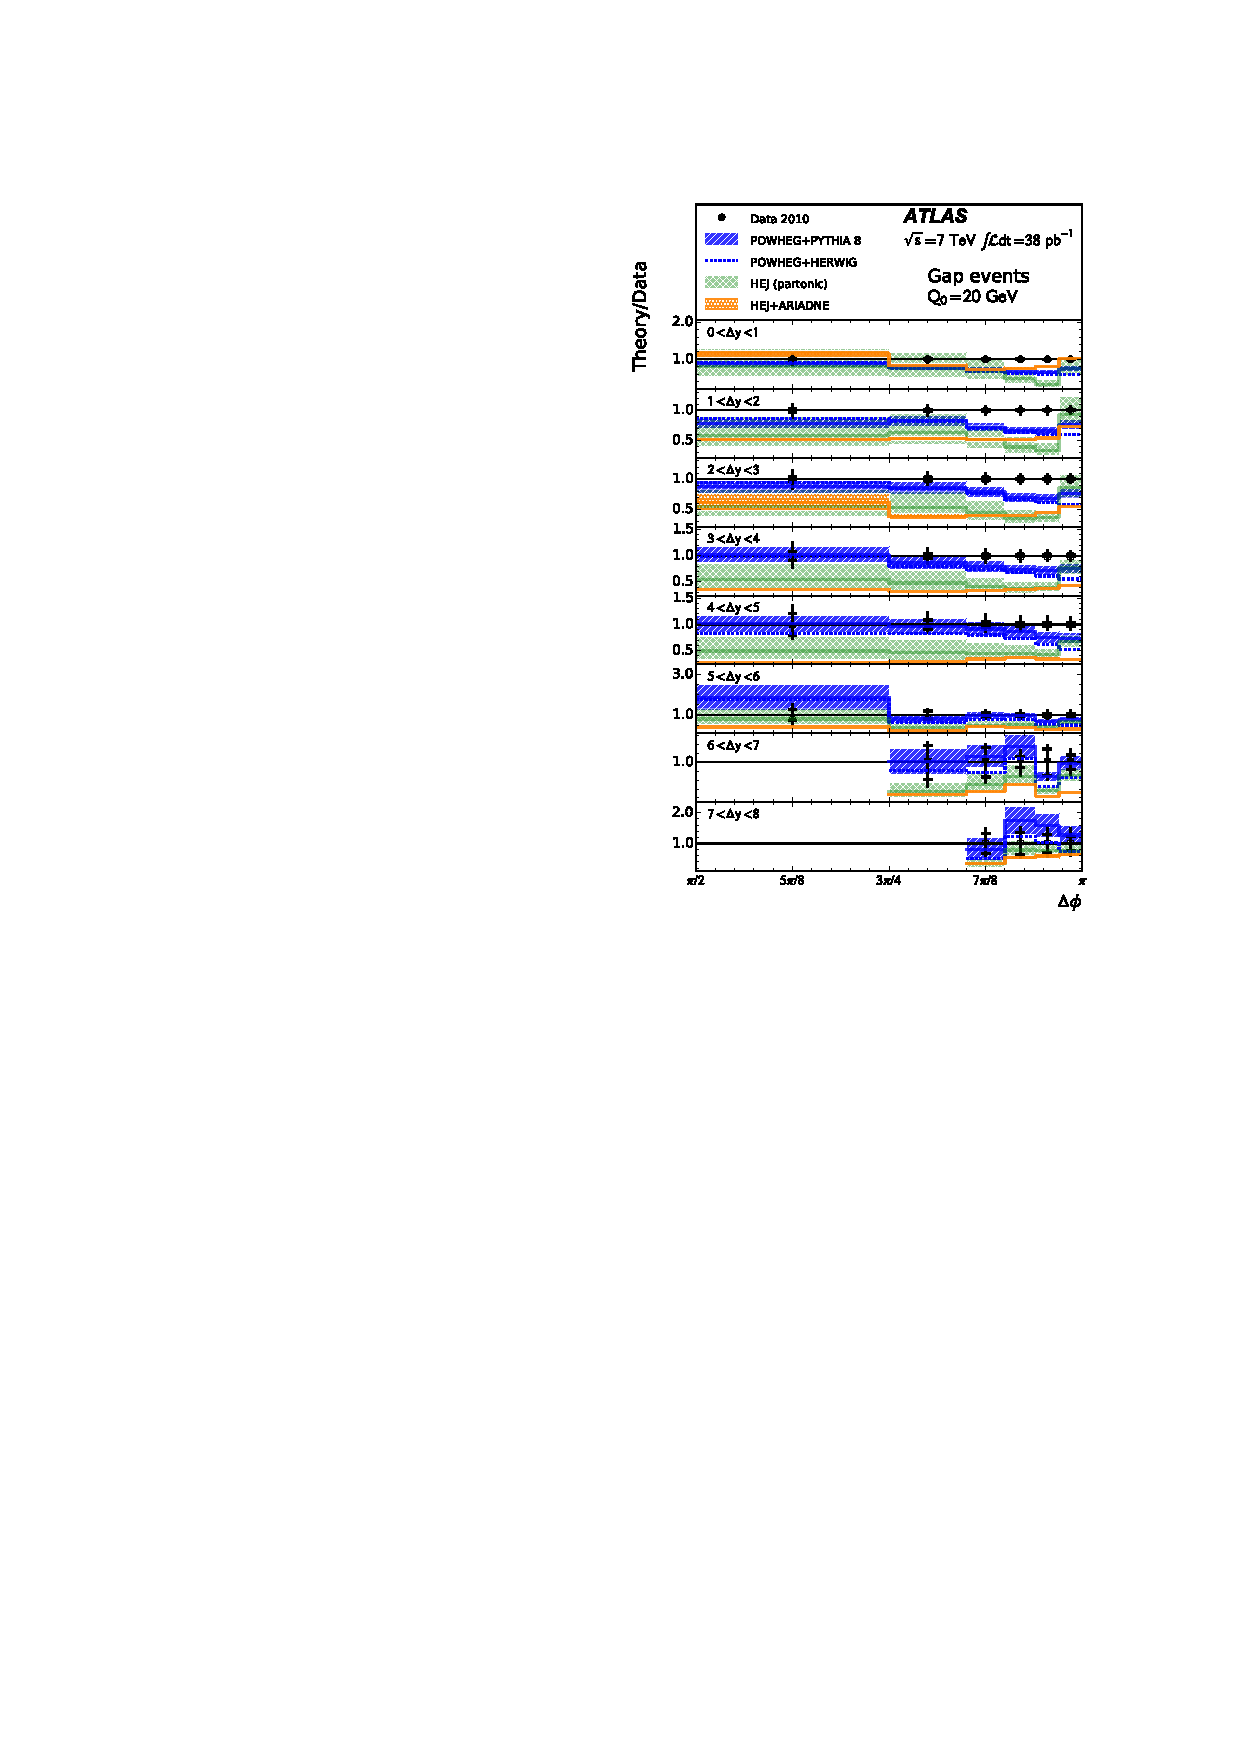
\includegraphics[width=\textwidth, height=1.0\textwidth]{pureJets8b}
			\caption{}
			\label{fig:}
		\end{subfigure}
		\caption{}
		\label{fig:}
	\end{figure}

\chapter{The $W^\pm$ to $\zg$ Ratio at \texttt{ATLAS}}
\label{chap:WZRatio}

Compare HEJ Z+Jets to NJet (NLO predictions) and MadGraph (LO predictions).  ***Is this still worth it? Data/HEJ/MG all very unstable...***

\chapter{$\zg$+Jets at 100TeV}
\label{chap:100TeV}

	\begin{itemize}
		\item Talk about the FCC movement and the effect we expect the resummation will have at these energies.
		\item Put all three lines (30GeV, 60GeV, 100GeV) on the same plots in this section?
		\item Pros: Can see that we can put more stringent cuts while maintaining x-section.  Also
		      makes the point that we can cut out all the NP physics we cant model.
		\item Cons: Plots will be very busy.
	\end{itemize}

	\begin{figure}[h]
		\centering
		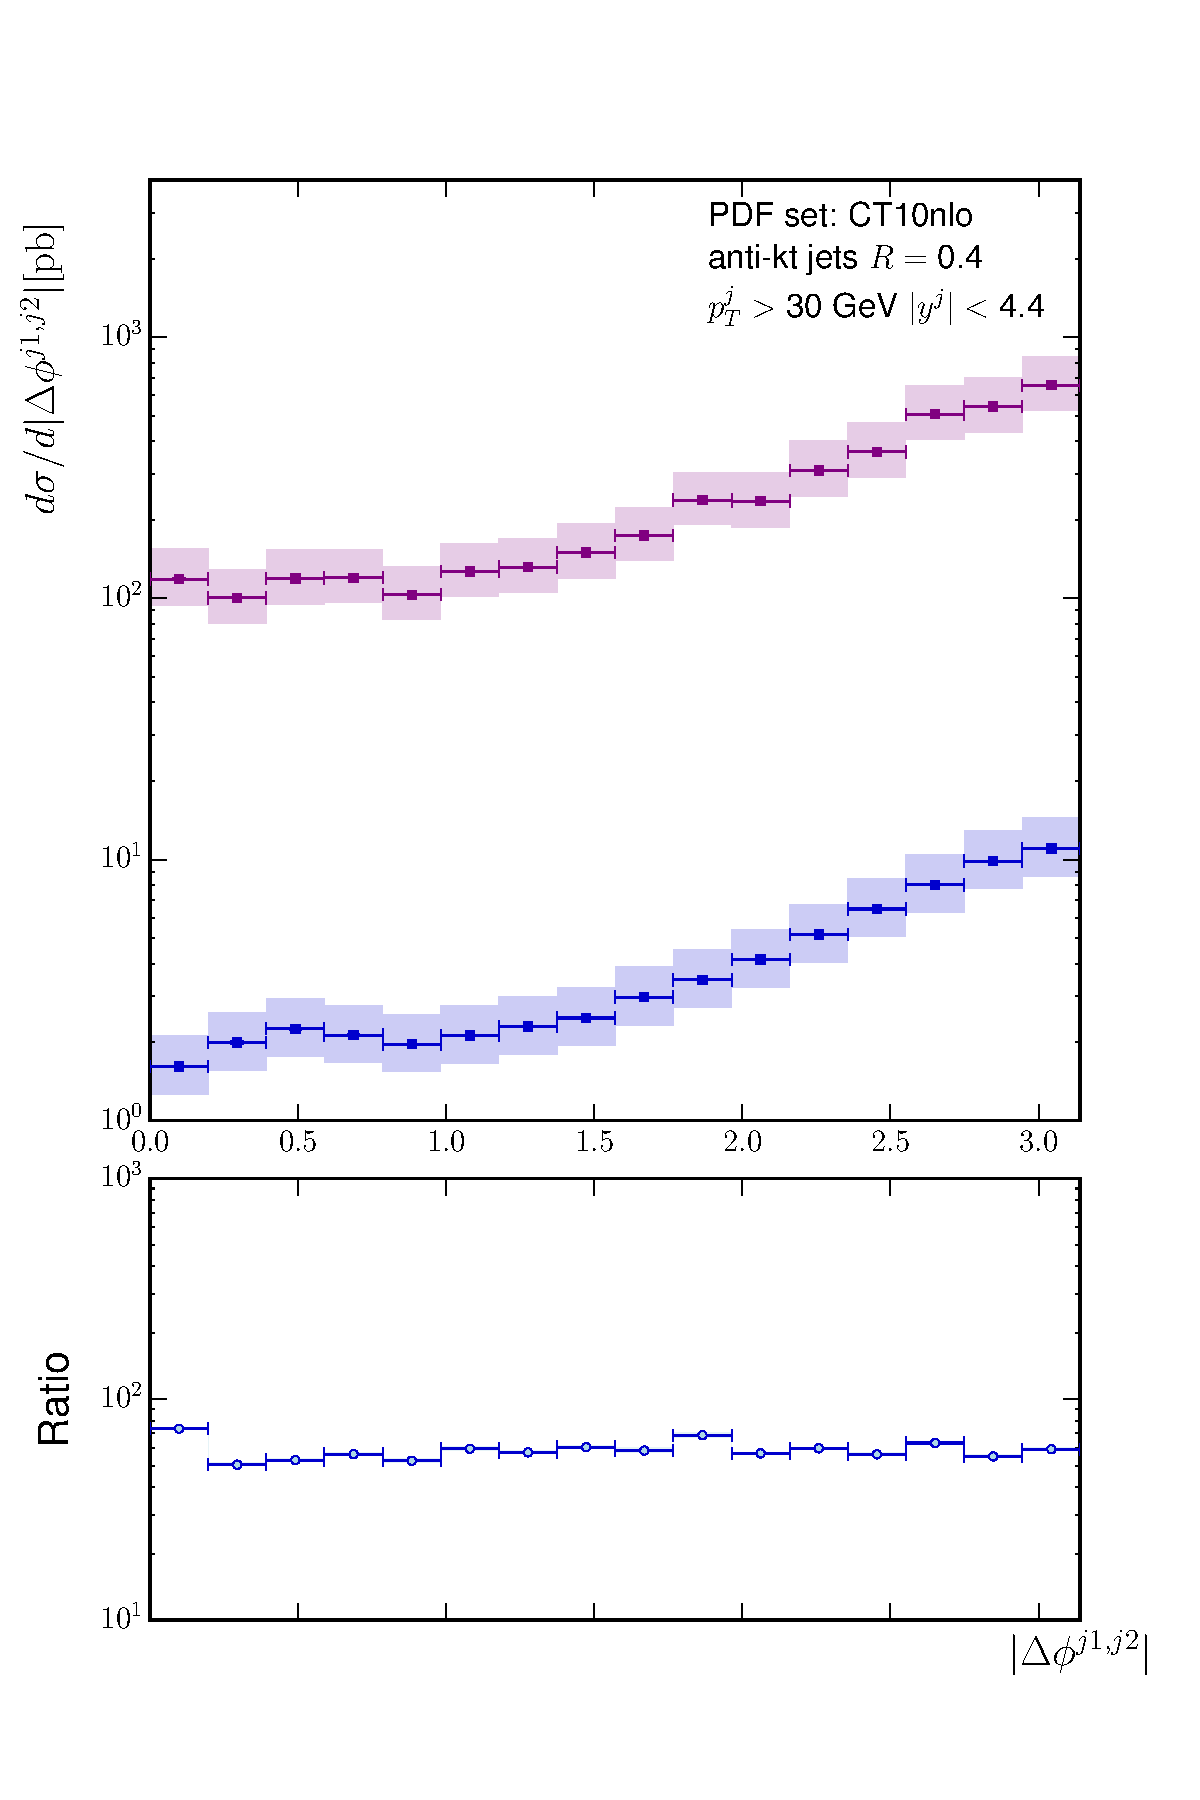
\includegraphics[width=0.8\linewidth]{ATLAS_Z_100TeV_12a}
		\caption{12a}
		\label{fig:100tev_12a}
	\end{figure}

	Figure (\ref{fig:100tev_12a}) notes:

	\begin{itemize}
		\item dphi plot
		\item Start with this one because its the most boring,
		\item i.e. if QCD didnt change with energy scale all plots would be like this one
	\end{itemize}

	\begin{figure}[h]
		\centering
		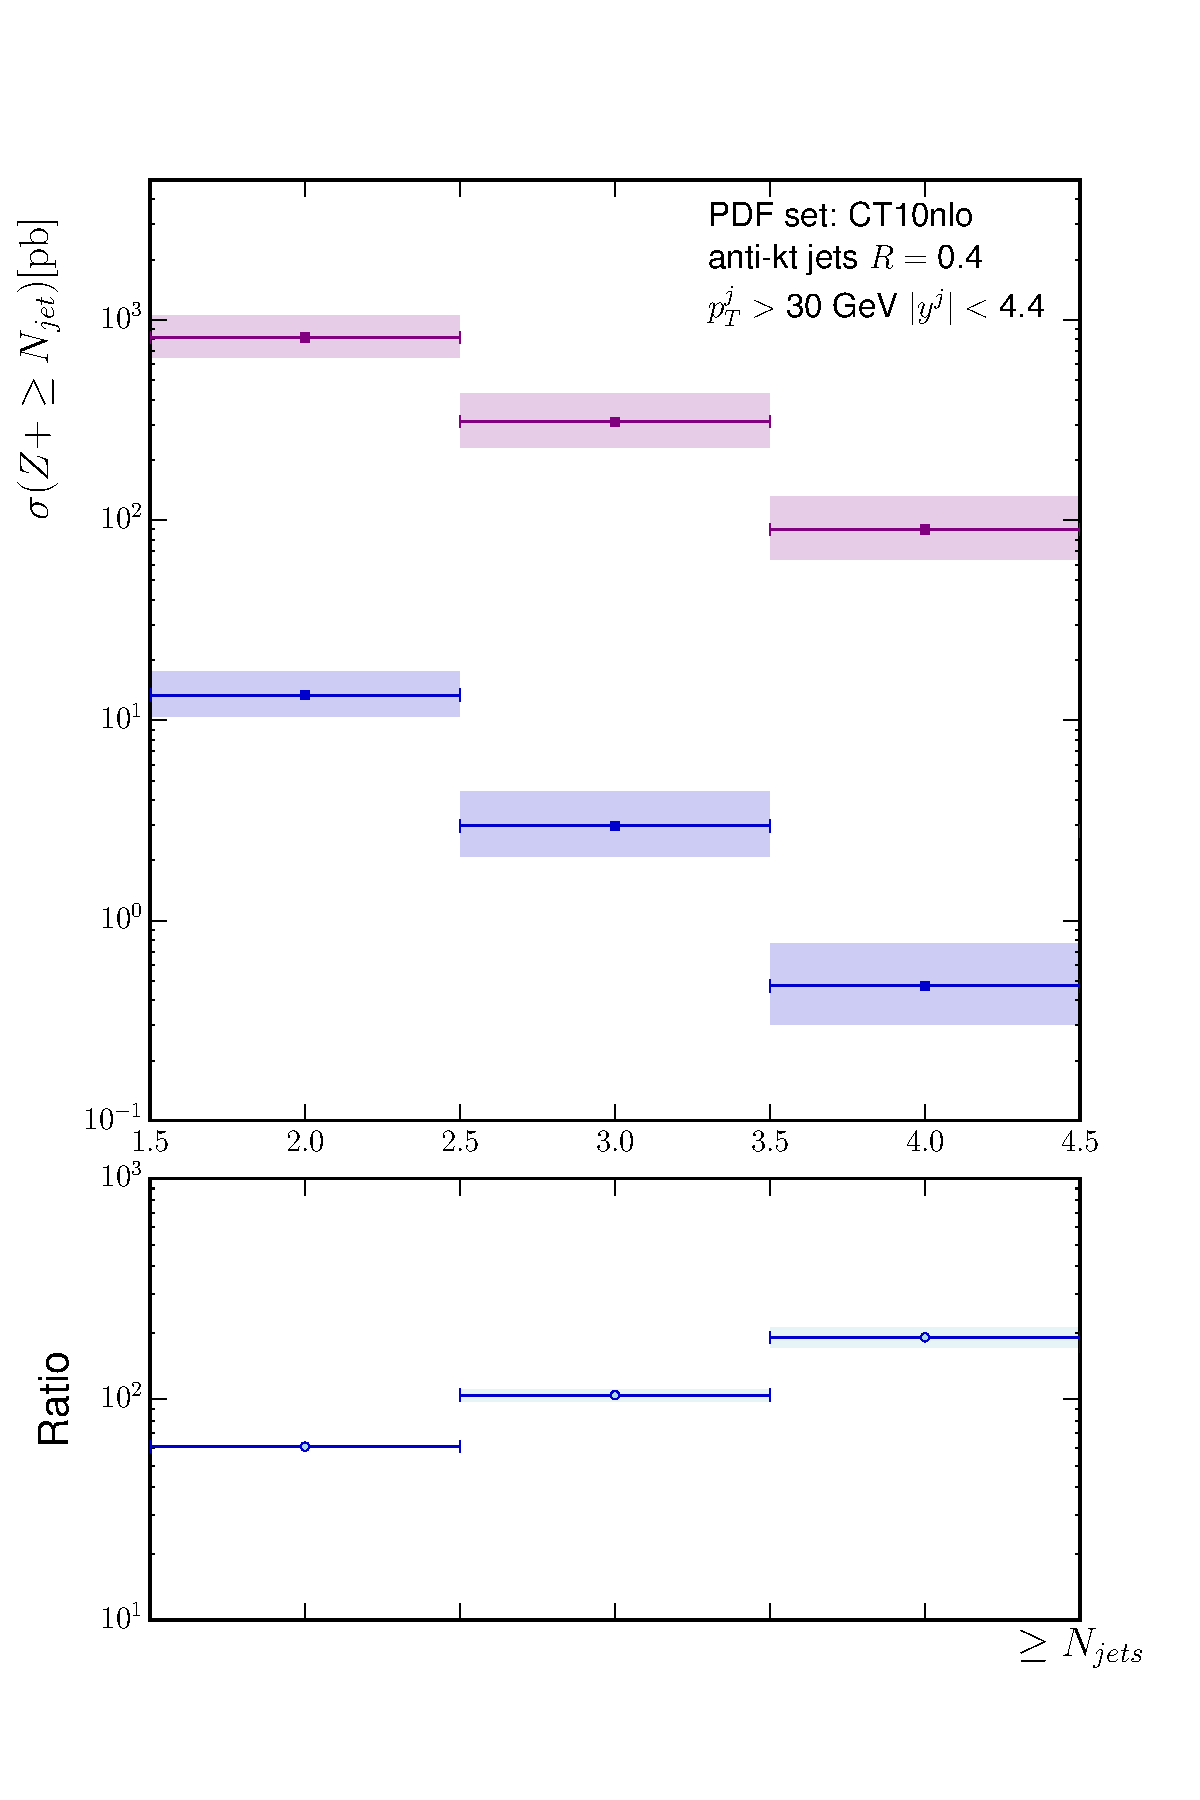
\includegraphics[width=0.8\linewidth]{ATLAS_Z_100TeV_2a}
		\caption{12a}
		\label{fig:100tev_2a}
	\end{figure}

	Figure (\ref{fig:100tev_2a}) notes:

	\begin{itemize}
		\item njets,
		\item Explicitly shows that the break-down of the perturbative series gets worse at higher energies,
		\item The contributions from higher-order corrections increase as the energy increases,
	\end{itemize}

	\begin{figure}[h]
		\centering
		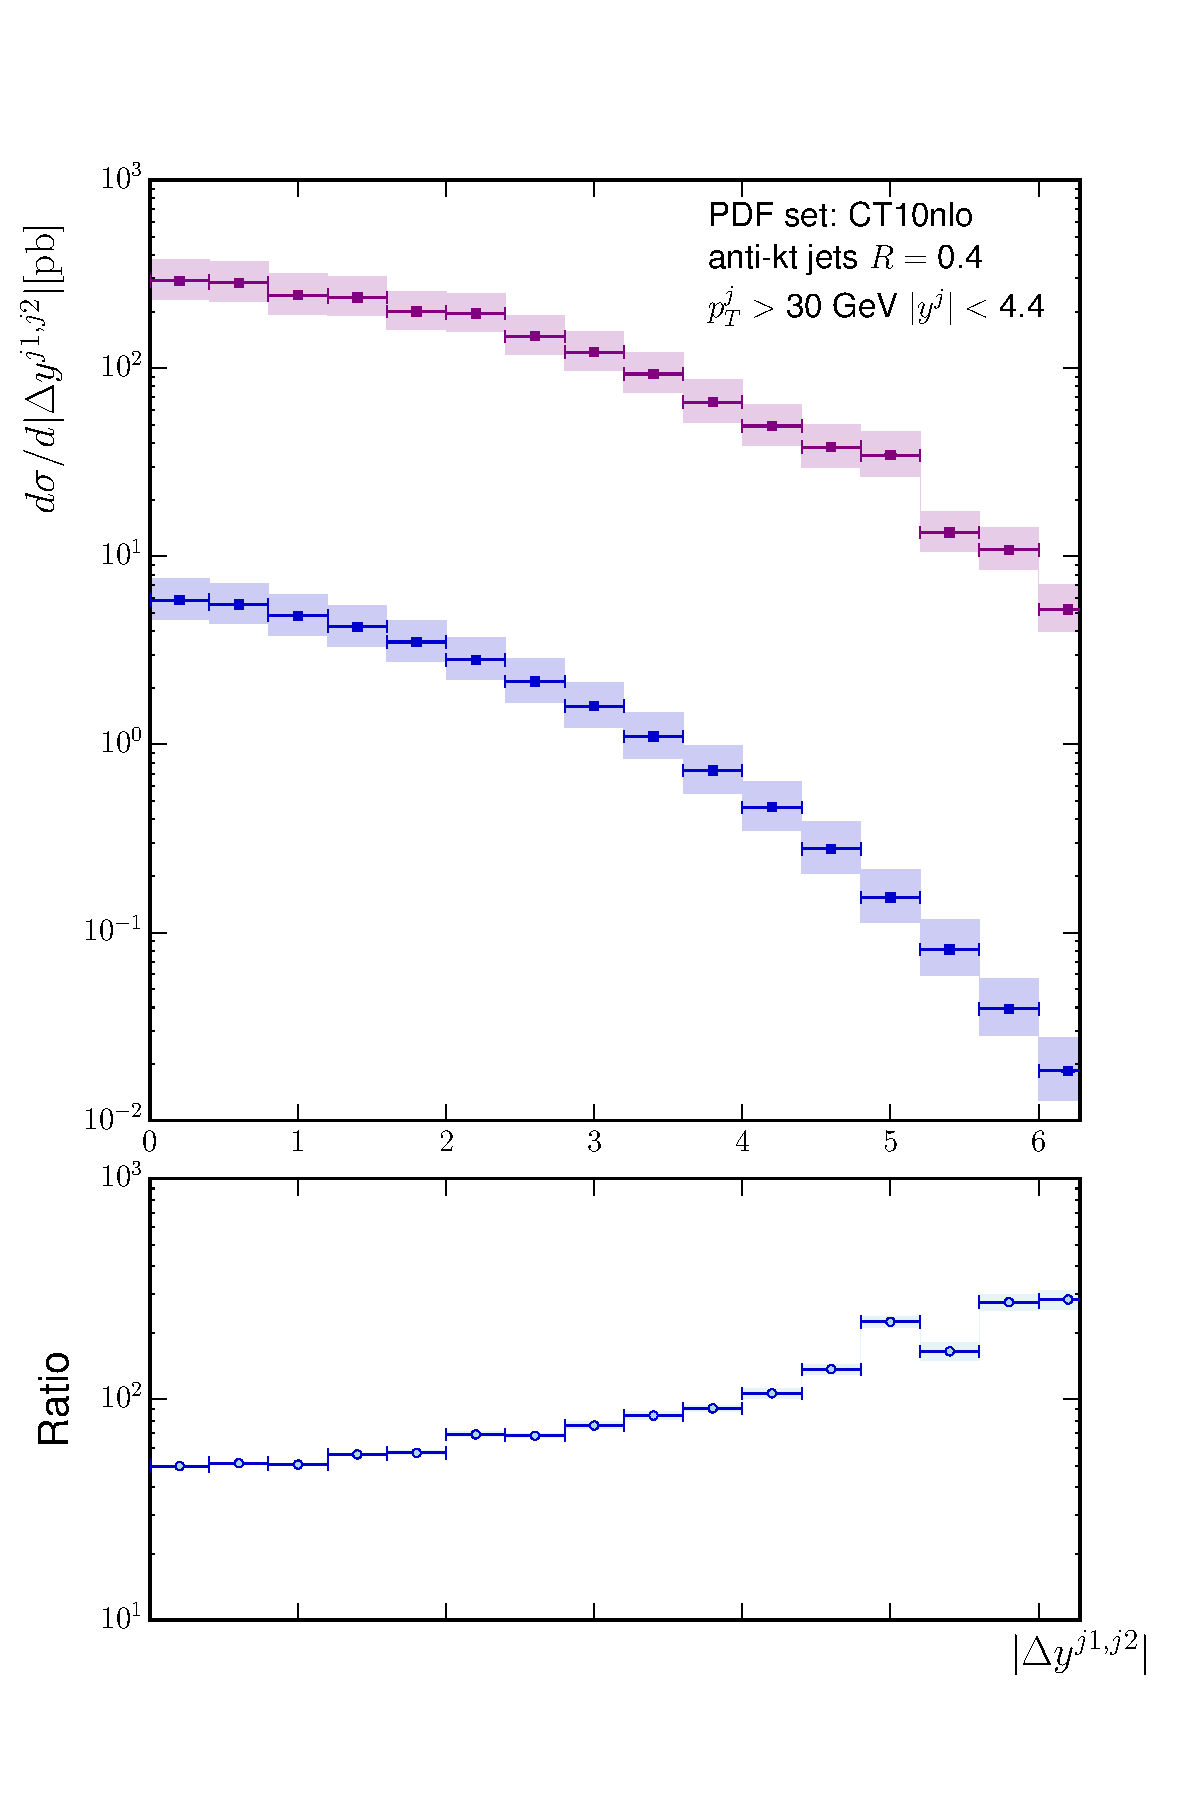
\includegraphics[width=0.8\linewidth]{ATLAS_Z_100TeV_11a}
		\caption{11a}
		\label{fig:100tev_11a}
	\end{figure}

	Figure (\ref{fig:100tev_11a}) notes:

	\begin{itemize}
		\item dy plot,
		\item O(10) increase in cross-section as we go to large rapidities,
		\item More energy in initial state means we can get more jets further in to the outer regions of y-space,
		\item The increase seen is \emph{exactly} the large logs we capture at play
	\end{itemize}

	\begin{figure}[h]
		\centering
		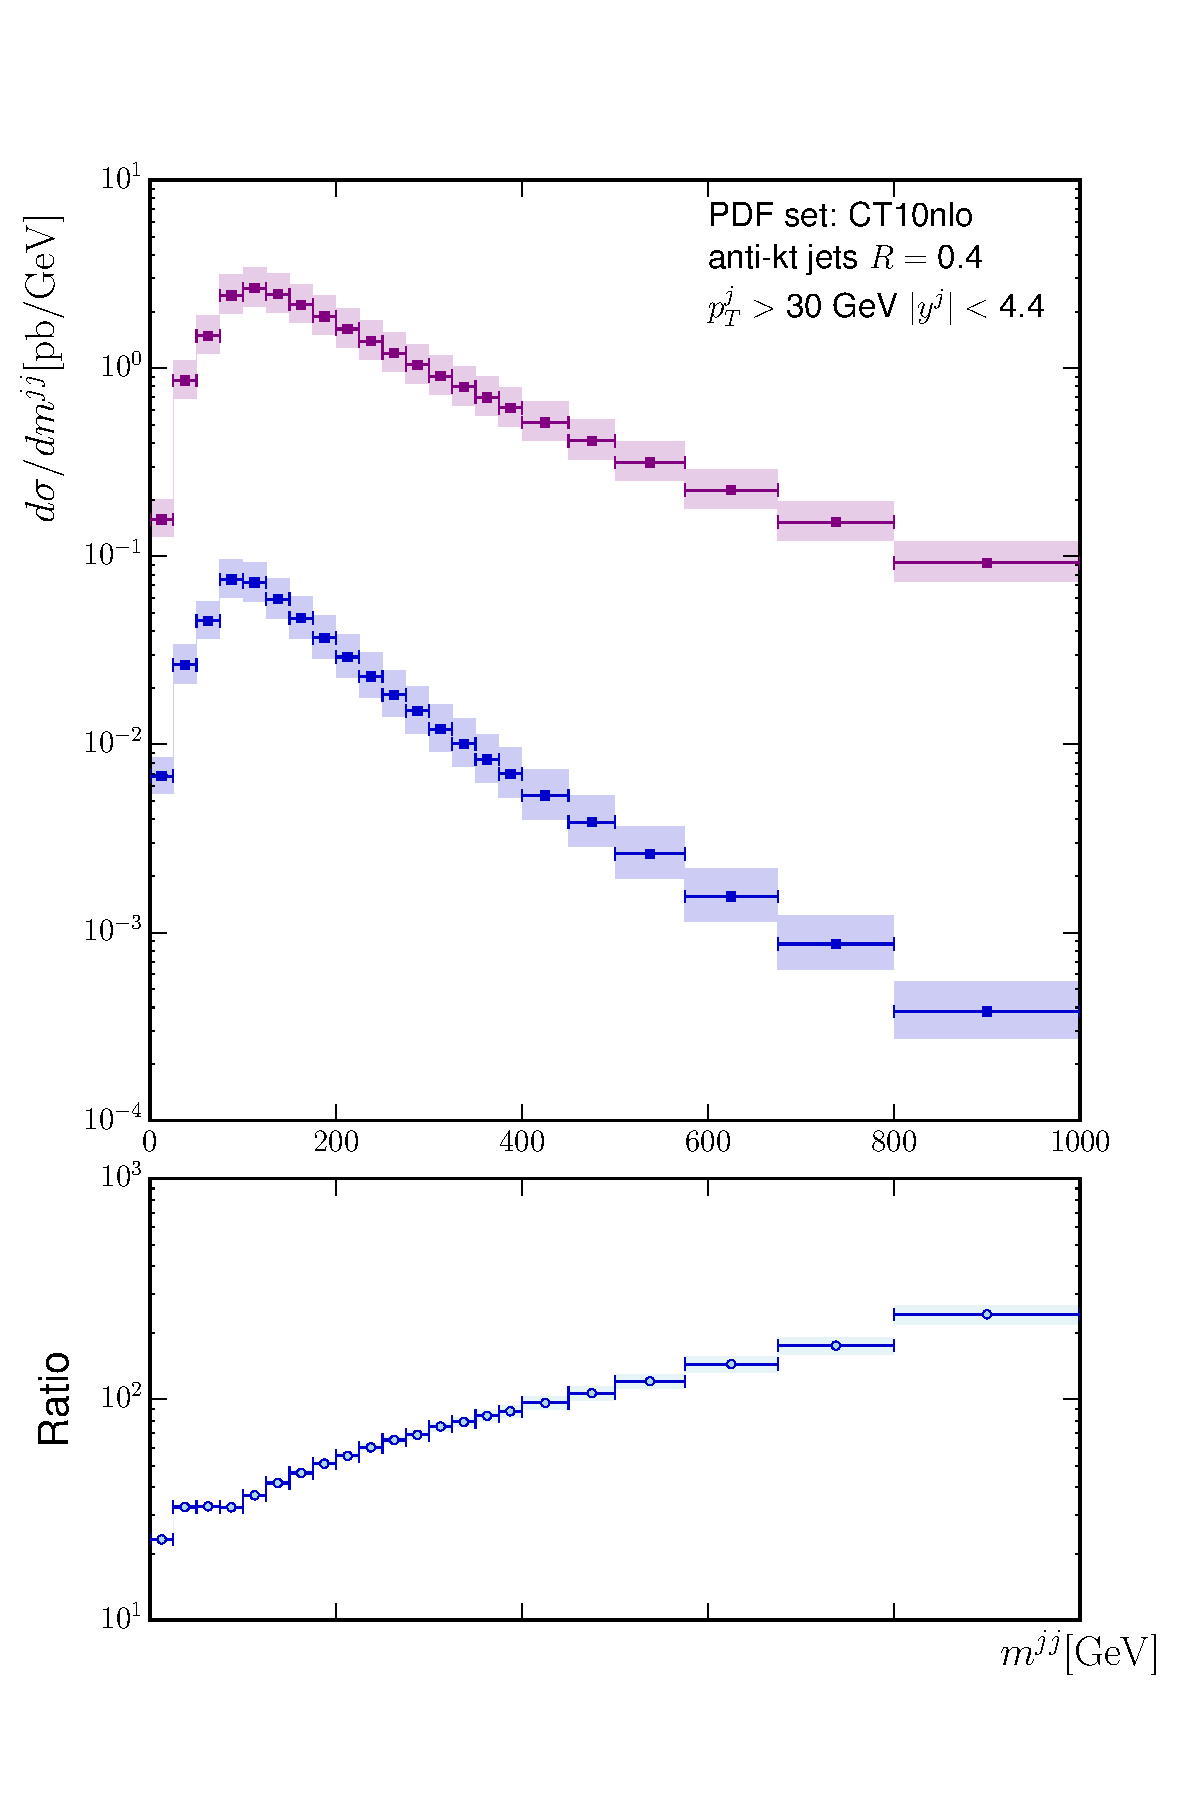
\includegraphics[width=0.8\linewidth]{ATLAS_Z_100TeV_11b}
		\caption{11b}
		\label{fig:100tev_11b}
	\end{figure}

	Figure (\ref{fig:100tev_11b}) notes:

	\begin{itemize}
		\item $dm_jj$ plot,
		\item O(10) increase in cross-section as we go to large invariant masses,
		\item Invariant masses again correlate with the logs we resum (show this explicitly if you havent already),
		\item Similar to figure (\ref{fig:100tev_11a})
	\end{itemize}

	\begin{figure}[h]
		\centering
		\begin{subfigure}[b]{0.48\textwidth}
			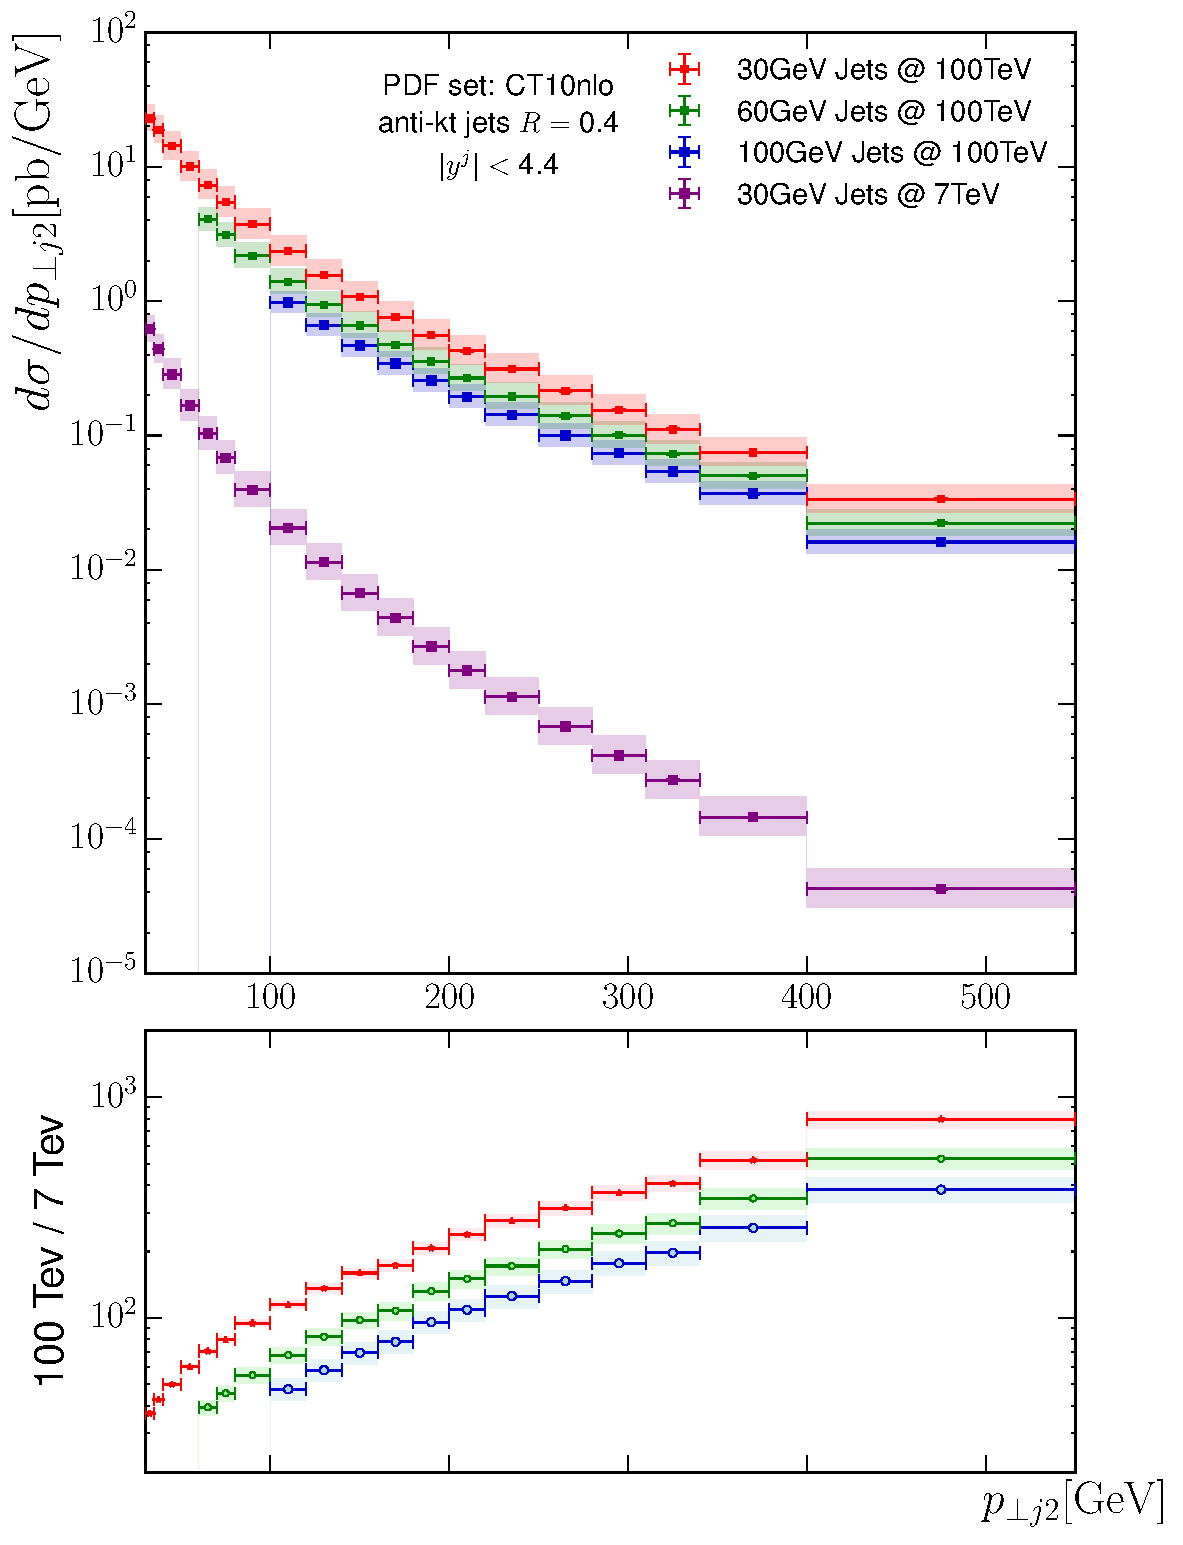
\includegraphics[width=\textwidth, height=1.3\textwidth]{ATLAS_Z_100TeV_5b}
			\caption{}
			\label{fig:100tev_5b}
		\end{subfigure}

		\begin{subfigure}[b]{0.48\textwidth}
			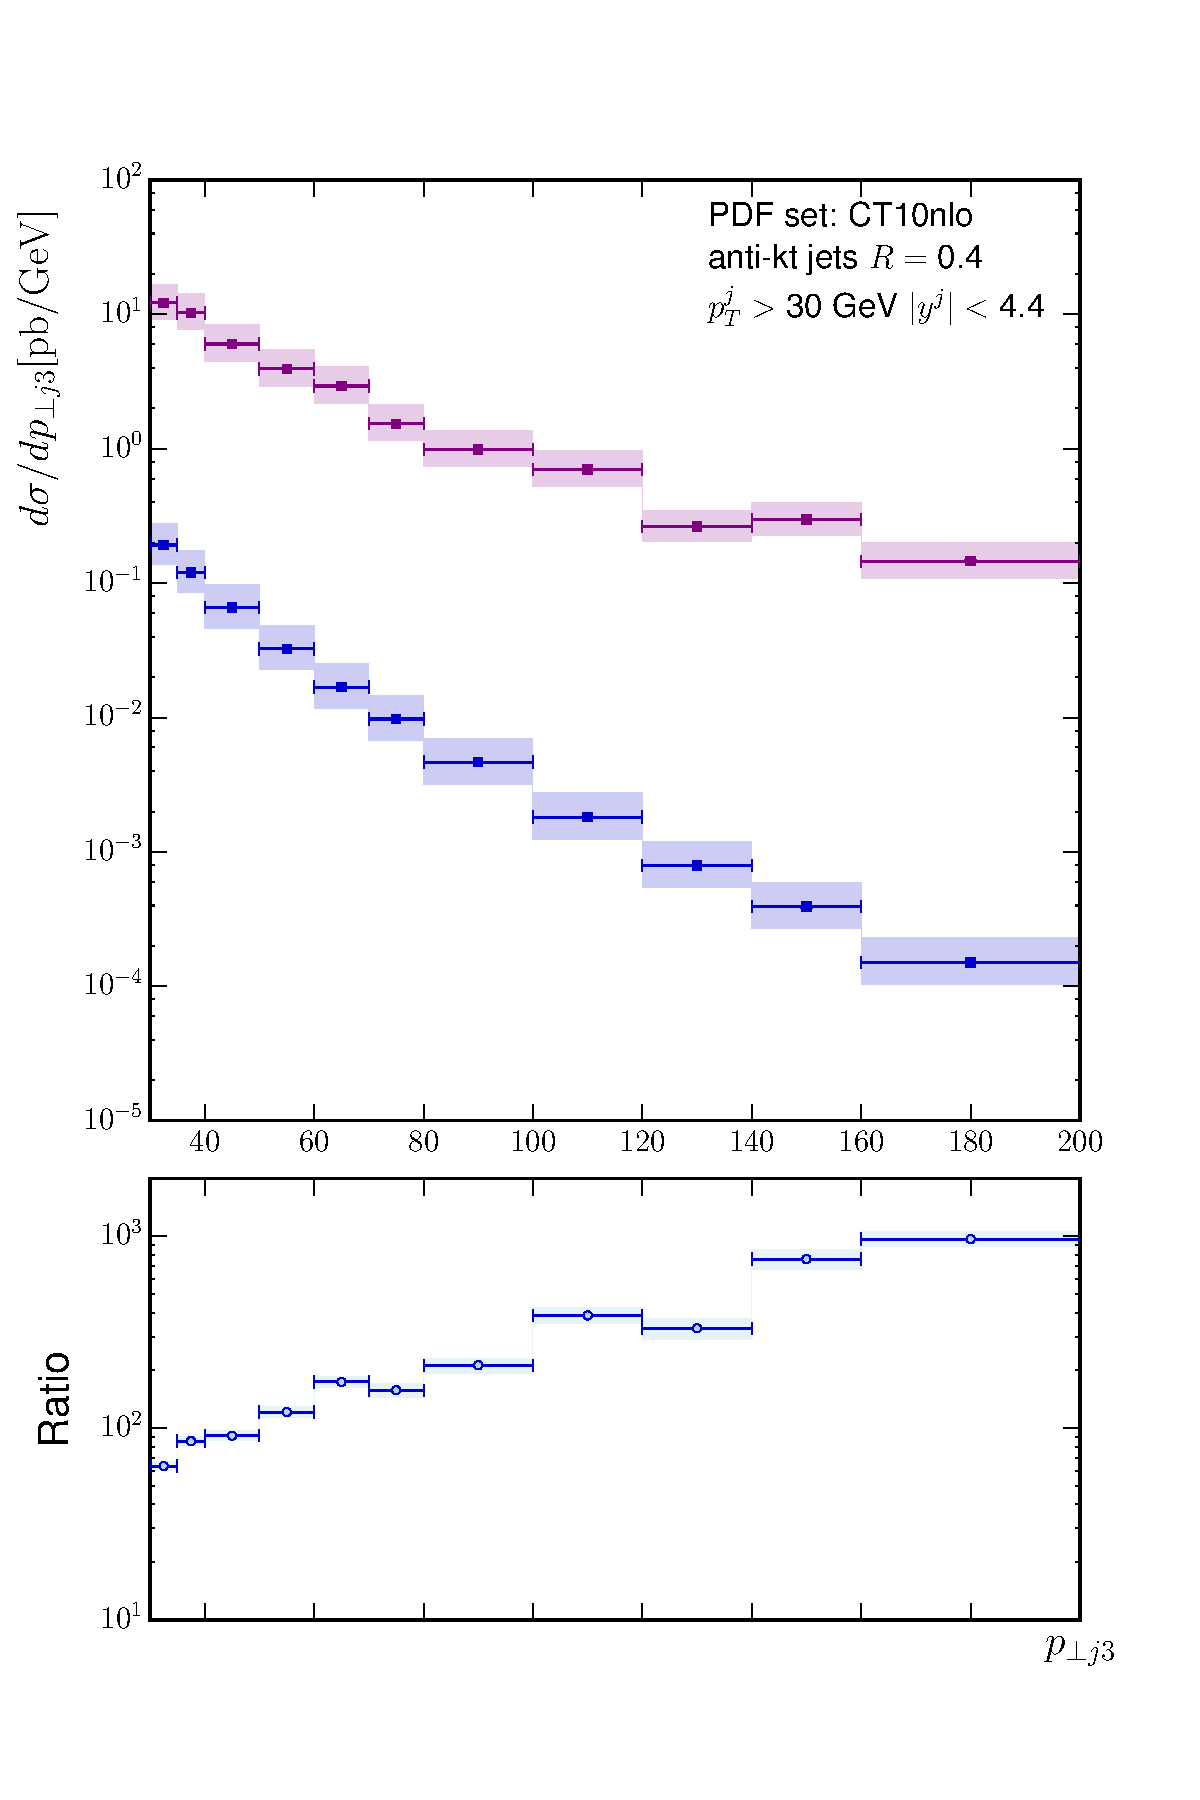
\includegraphics[width=\textwidth, height=1.3\textwidth]{ATLAS_Z_100TeV_6a}
			\caption{}
			\label{fig:100tev_6a}
		\end{subfigure}
		~
		\begin{subfigure}[b]{0.48\textwidth}
			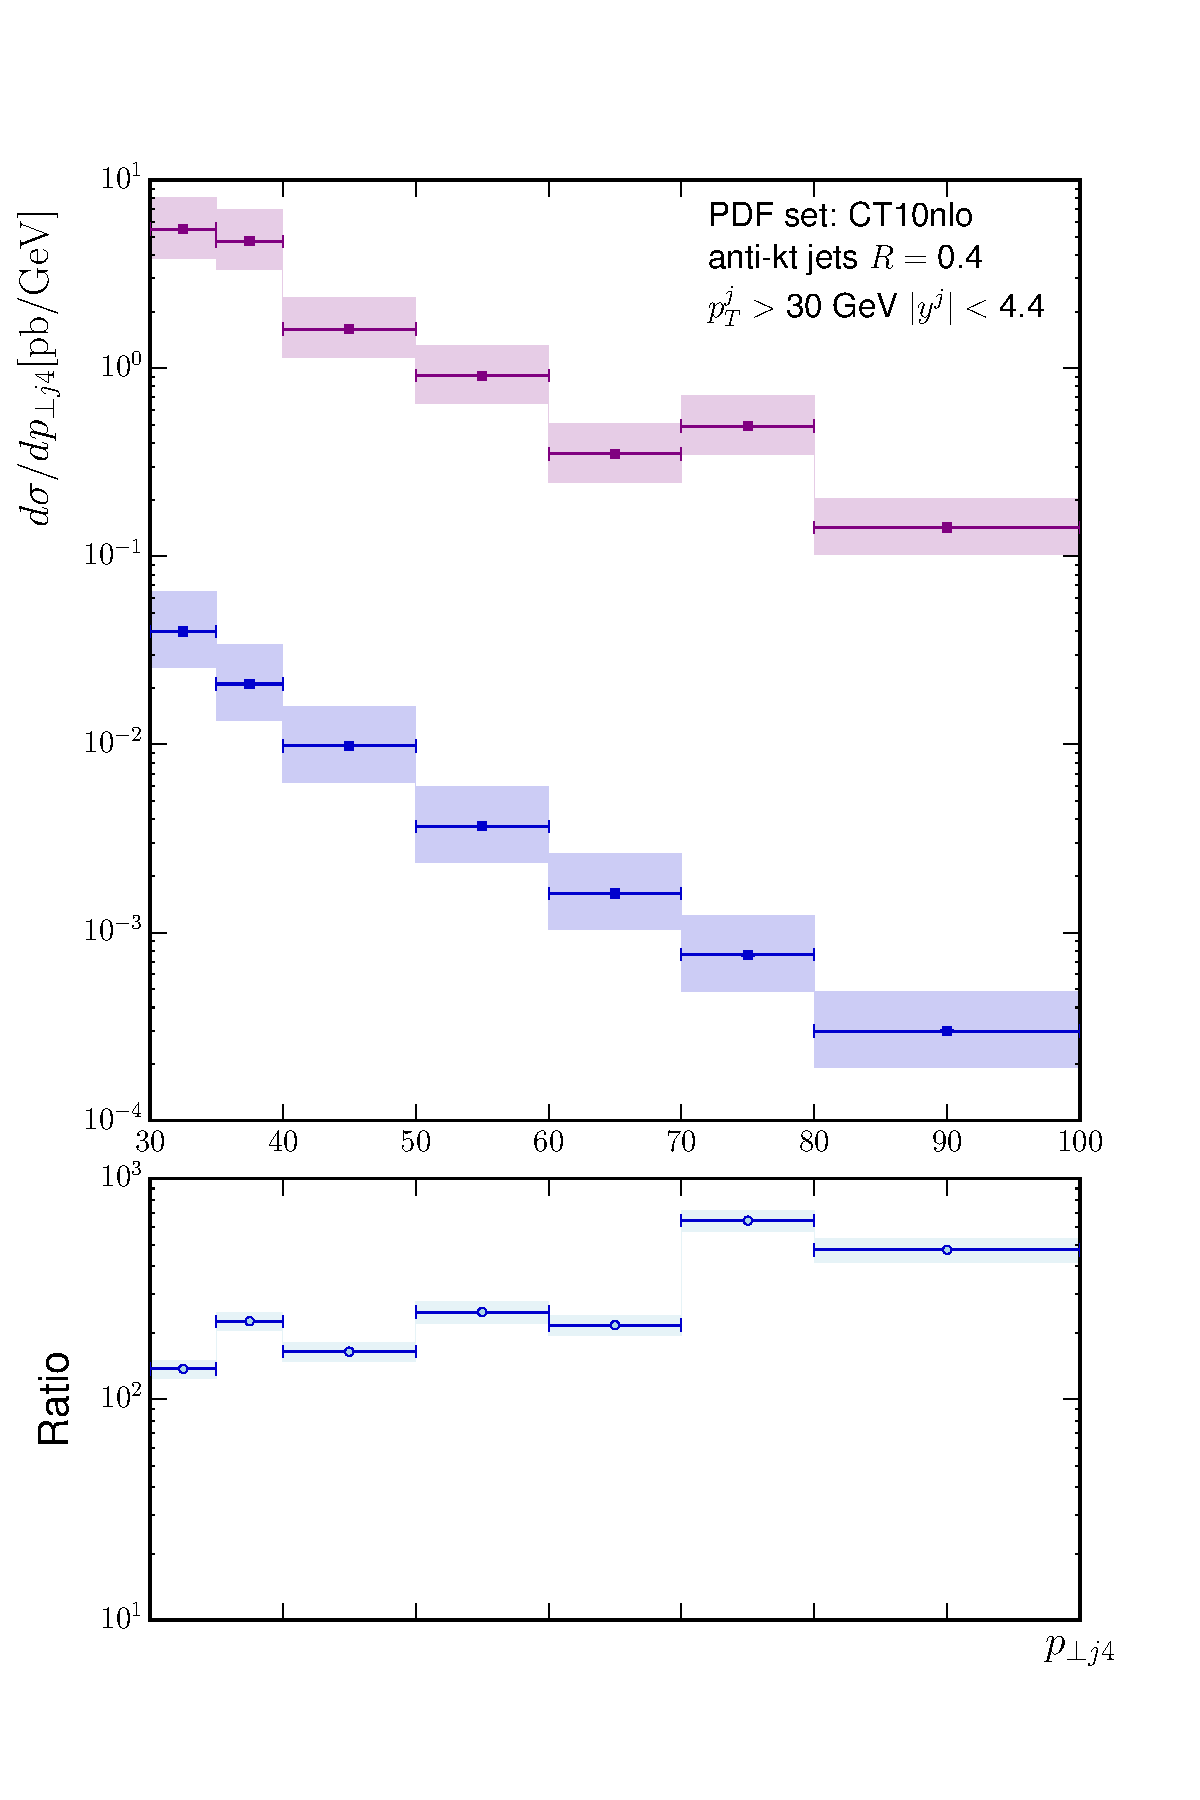
\includegraphics[width=\textwidth, height=1.3\textwidth]{ATLAS_Z_100TeV_6b}
			\caption{}
			\label{fig:100tev_6b}
		\end{subfigure}
		\caption{}
	\end{figure}

	Figure (\ref{fig:100tev_5b}-\ref{fig:100tev_6b}) notes:

	\begin{itemize}
		\item pT distributions,
		\item Heavy tails...soooo?
		\item More energy in initial state means we can get more jets further in to the outer regions of y-space,
		\item What effect would a shower have on these distributions?  Plenty of spare pT to radiate.
	\end{itemize}

	\begin{figure}[h]
		\centering
		\begin{subfigure}[b]{0.48\textwidth}
			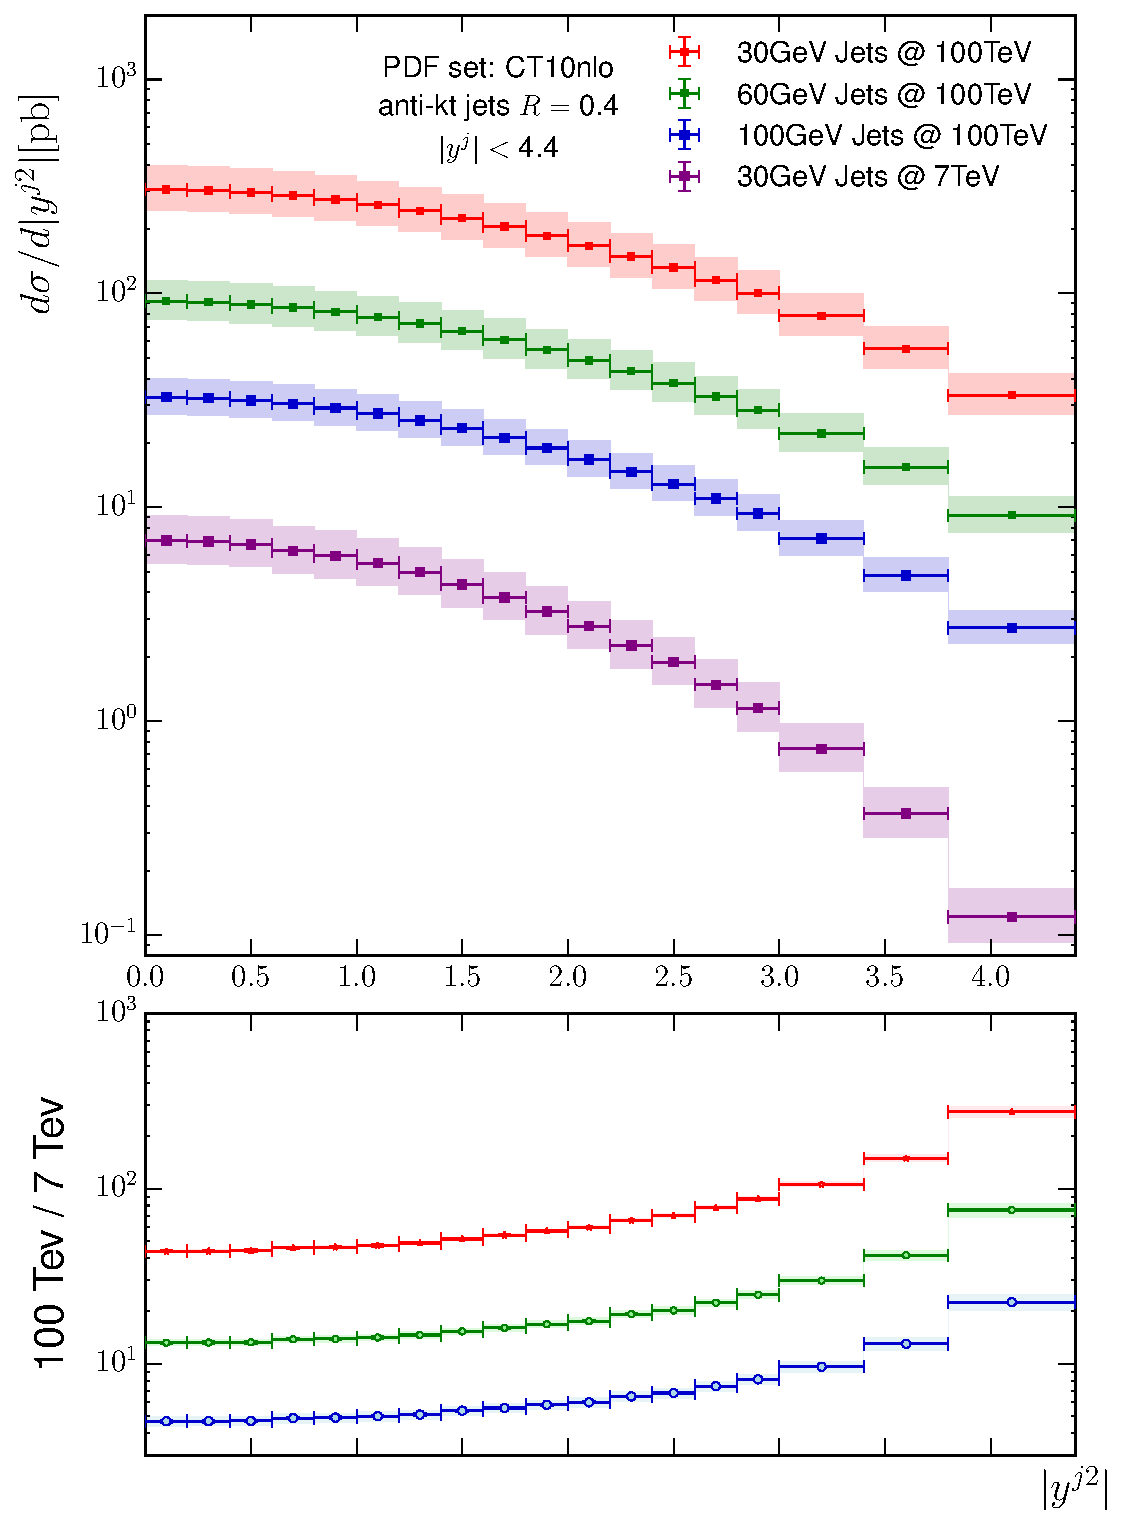
\includegraphics[width=\textwidth, height=1.3\textwidth]{ATLAS_Z_100TeV_9b}
			\caption{}
			\label{fig:100tev_9b}
		\end{subfigure}

		\begin{subfigure}[b]{0.48\textwidth}
			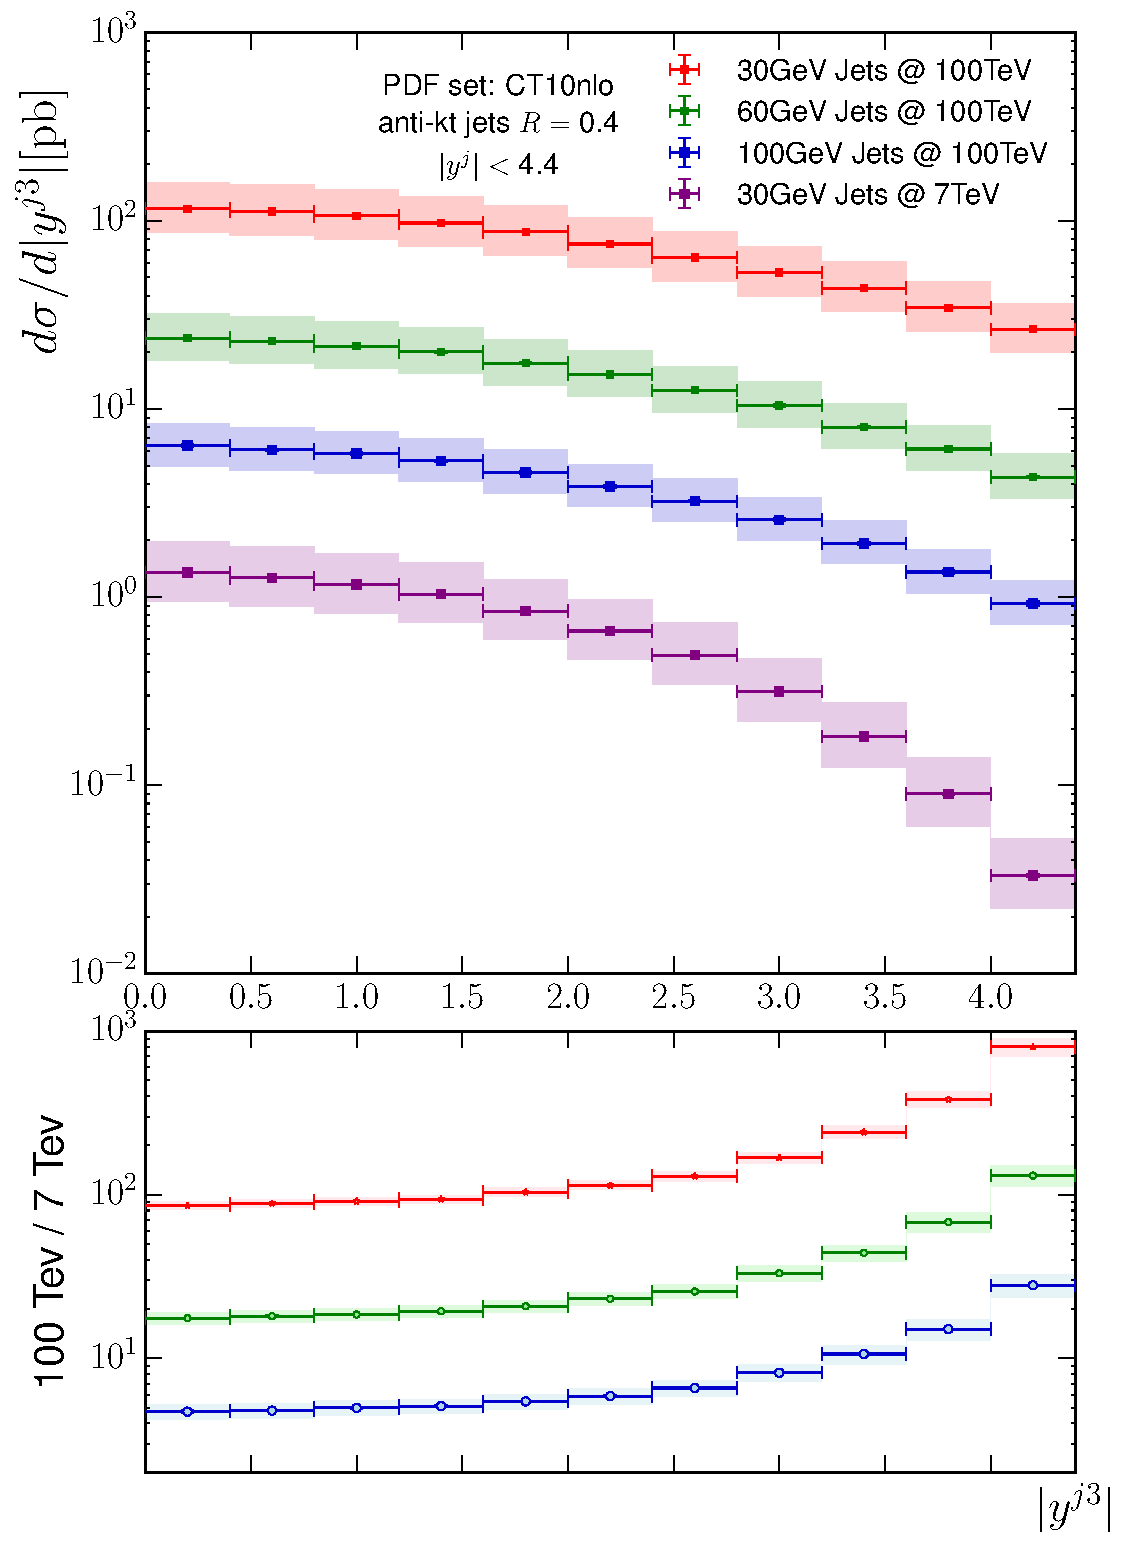
\includegraphics[width=\textwidth, height=1.3\textwidth]{ATLAS_Z_100TeV_10a}
			\caption{}
			\label{fig:100tev_10a}
		\end{subfigure}
		~
		\begin{subfigure}[b]{0.48\textwidth}
			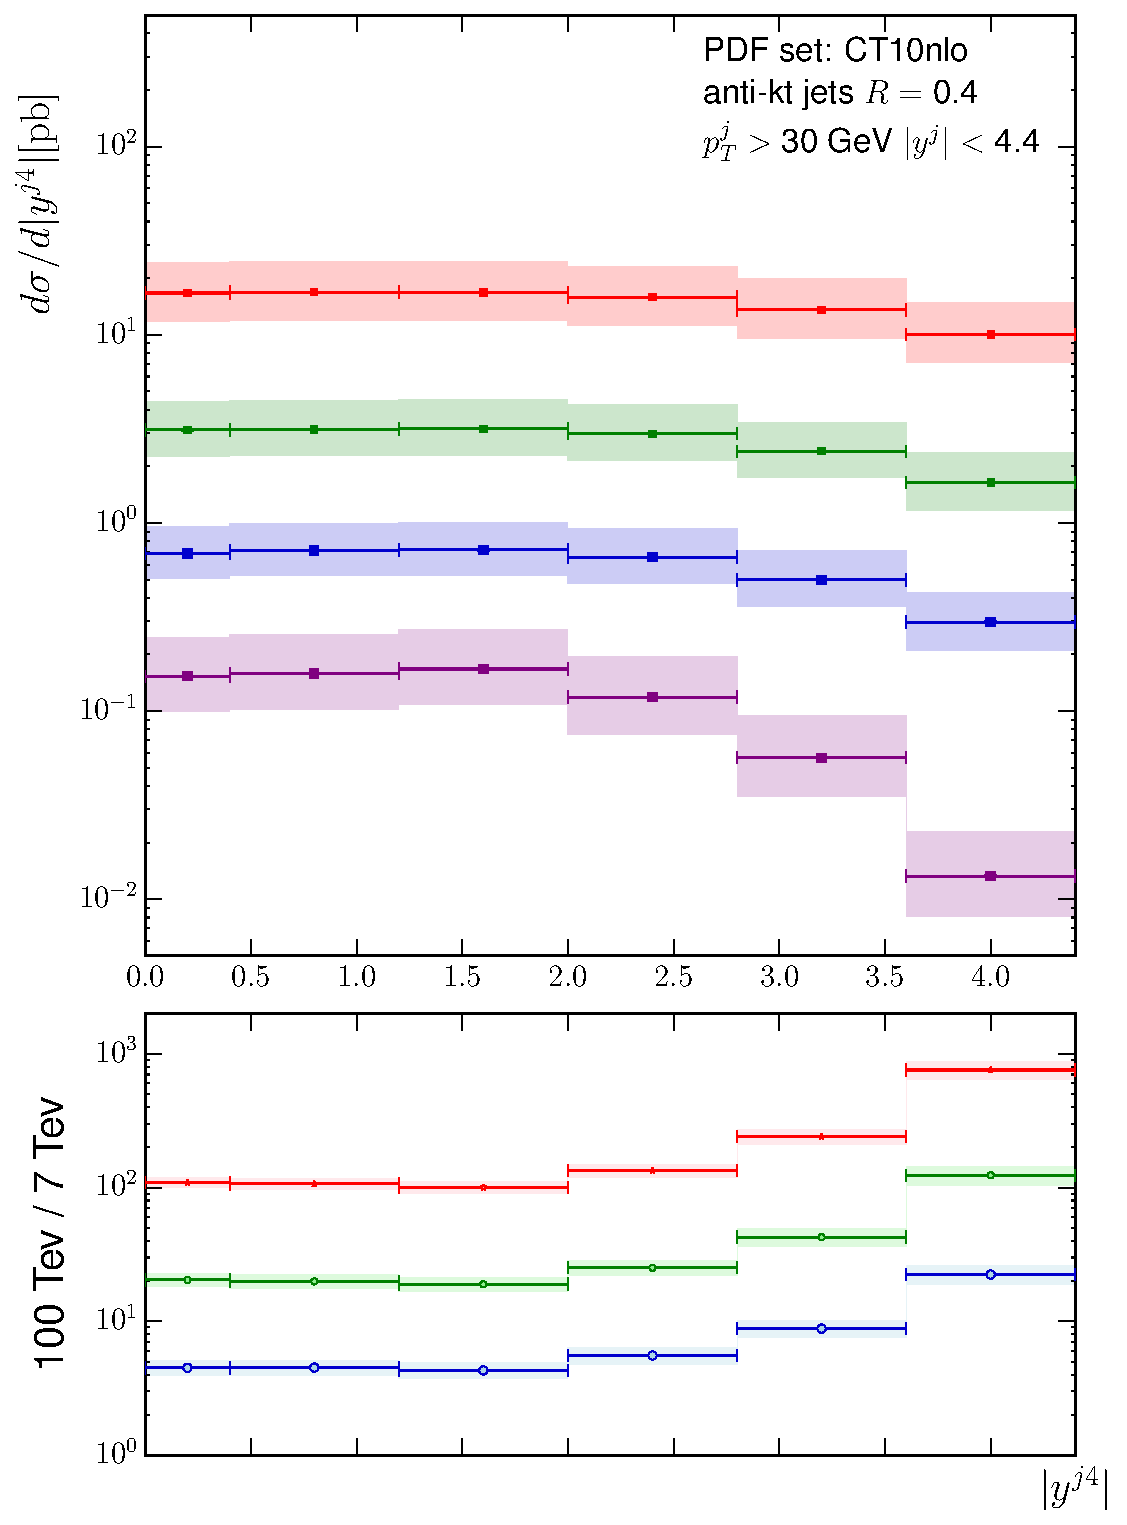
\includegraphics[width=\textwidth, height=1.3\textwidth]{ATLAS_Z_100TeV_10b}
			\caption{}
			\label{fig:100tev_10b}
		\end{subfigure}
		\caption{}
	\end{figure}

	Figure (\ref{fig:100tev_9b}-\ref{fig:100tev_10b}) notes:

	\begin{itemize}
		\item Not much more to say about these - mostly covered in dy plots,
	\end{itemize}

